\chapter{Implementation}
\label{chapter:implementation}

In chapter 3, it was presented an overview of the SmartLighting project, giving an outline of the requirements and use cases. Also, to satisfy the project needs, an overview of the several scenarios of functioning as well as a possible architecture for the system was presented.

The objective for this chapter is to describe the steps and decisions taken, and the reasoning behind the implemented features. It starts in section \ref{implementation:objectives}, by presenting the objectives for the implementation, following by the used technologies on the several components in section \ref{implementation:technologies}. After that, in sections \ref{implementation:devices} and \ref{implementation:rules}, it is presented the standards used to access the devices and to define rules, respectively. Following, in section \ref{implementation:architecture}, the whole system's architecture as well as the functioning of its components is described. 

Since one of the requirements and objectives for this project was the existence of failure handling mechanisms, in section \ref{implementation:scenarios}, it is described the implementation taking into account the several scenarios addressed in the previous chapter. 

\newpage

\section{Objectives}
\label{implementation:objectives}

Although the implementation of the whole solution, presented in chapter \ref{chapter:architecture}, would be optimal to validate the project, it would be unrealistic due to the amount of time necessary to do so and the limited time available for this dissertation. Since some of the features were already implemented, such as a working platform to create and manage rules, a \ac{cep} engine and a simple gateway to communicate with devices through BLE, this dissertation's main focus was in the implementation of gateways capable of implement automation rules, alike to the ones implemented by the CEP engine, as well as give them means to adapt to failing and emergency states. For that reason, was also implemented a gateway manager to act as a monitor for the gateways, being able to control not only the functioning of each one of them as well as manage the distribution of rules and devices throughout the gateways.

Looking at the architecture presented in chapter 3, the component for the user management dashboard was not implemented for the scope of this work. Apart from this, all the features mentioned were implemented and are detailed in the continuation of this chapter.



\section{Adopted  Technologies}
\label{implementation:technologies}

This section aims to discuss the technologies chosen for the different components of the architecture. This choices will be explained taking into account the requirements for this project, however, it is important to note that there are no perfect solutions and, in some cases, several approaches could have been taken.

Since there was a dissertation that already implemented some features like the \ac{cep} engine and the \ac{bm}, some of the technologies used in this dissertation were influenced by past decisions. As far as the \ac{cep} engine concerns, the choice was the WSO2 \ac{cep} \cite{wso2}, since its features addressed all requirements, that such system would need, to fit this project's requirements. For the purpose of this dissertation both the \ac{cep} engine and the \ac{bm} as well as the communication between them, did not affect any of the new implemented features, however, since MQTT was primarily used as the elect protocol for communications in the referred dissertation, the implemented features presented in this work followed the same path.

Finally, it is important to state that the standard used, in SmartLighting project, for both object definition to read and write information to/from devices, and the rules structure, were also maintained and will be described in the following sections. 

\section{Access to Devices}
\label{implementation:devices}

Devices like sensors, which measure environment changes, and actuators, that trigger mechanisms to make changes in that same environment, are fundamental pieces to implement a smart and automated environment. Since there are a huge variety of devices with different characteristics, in order to enable extensibility for the system, the access to those devices, as well as the messages format, should be standardised. In another dissertation for this project, a standard following the IP Smart Objects Alliance guidelines was made and is illustrated in Figure \ref{fig:obj}

\begin{figure}[H]
	\centering
	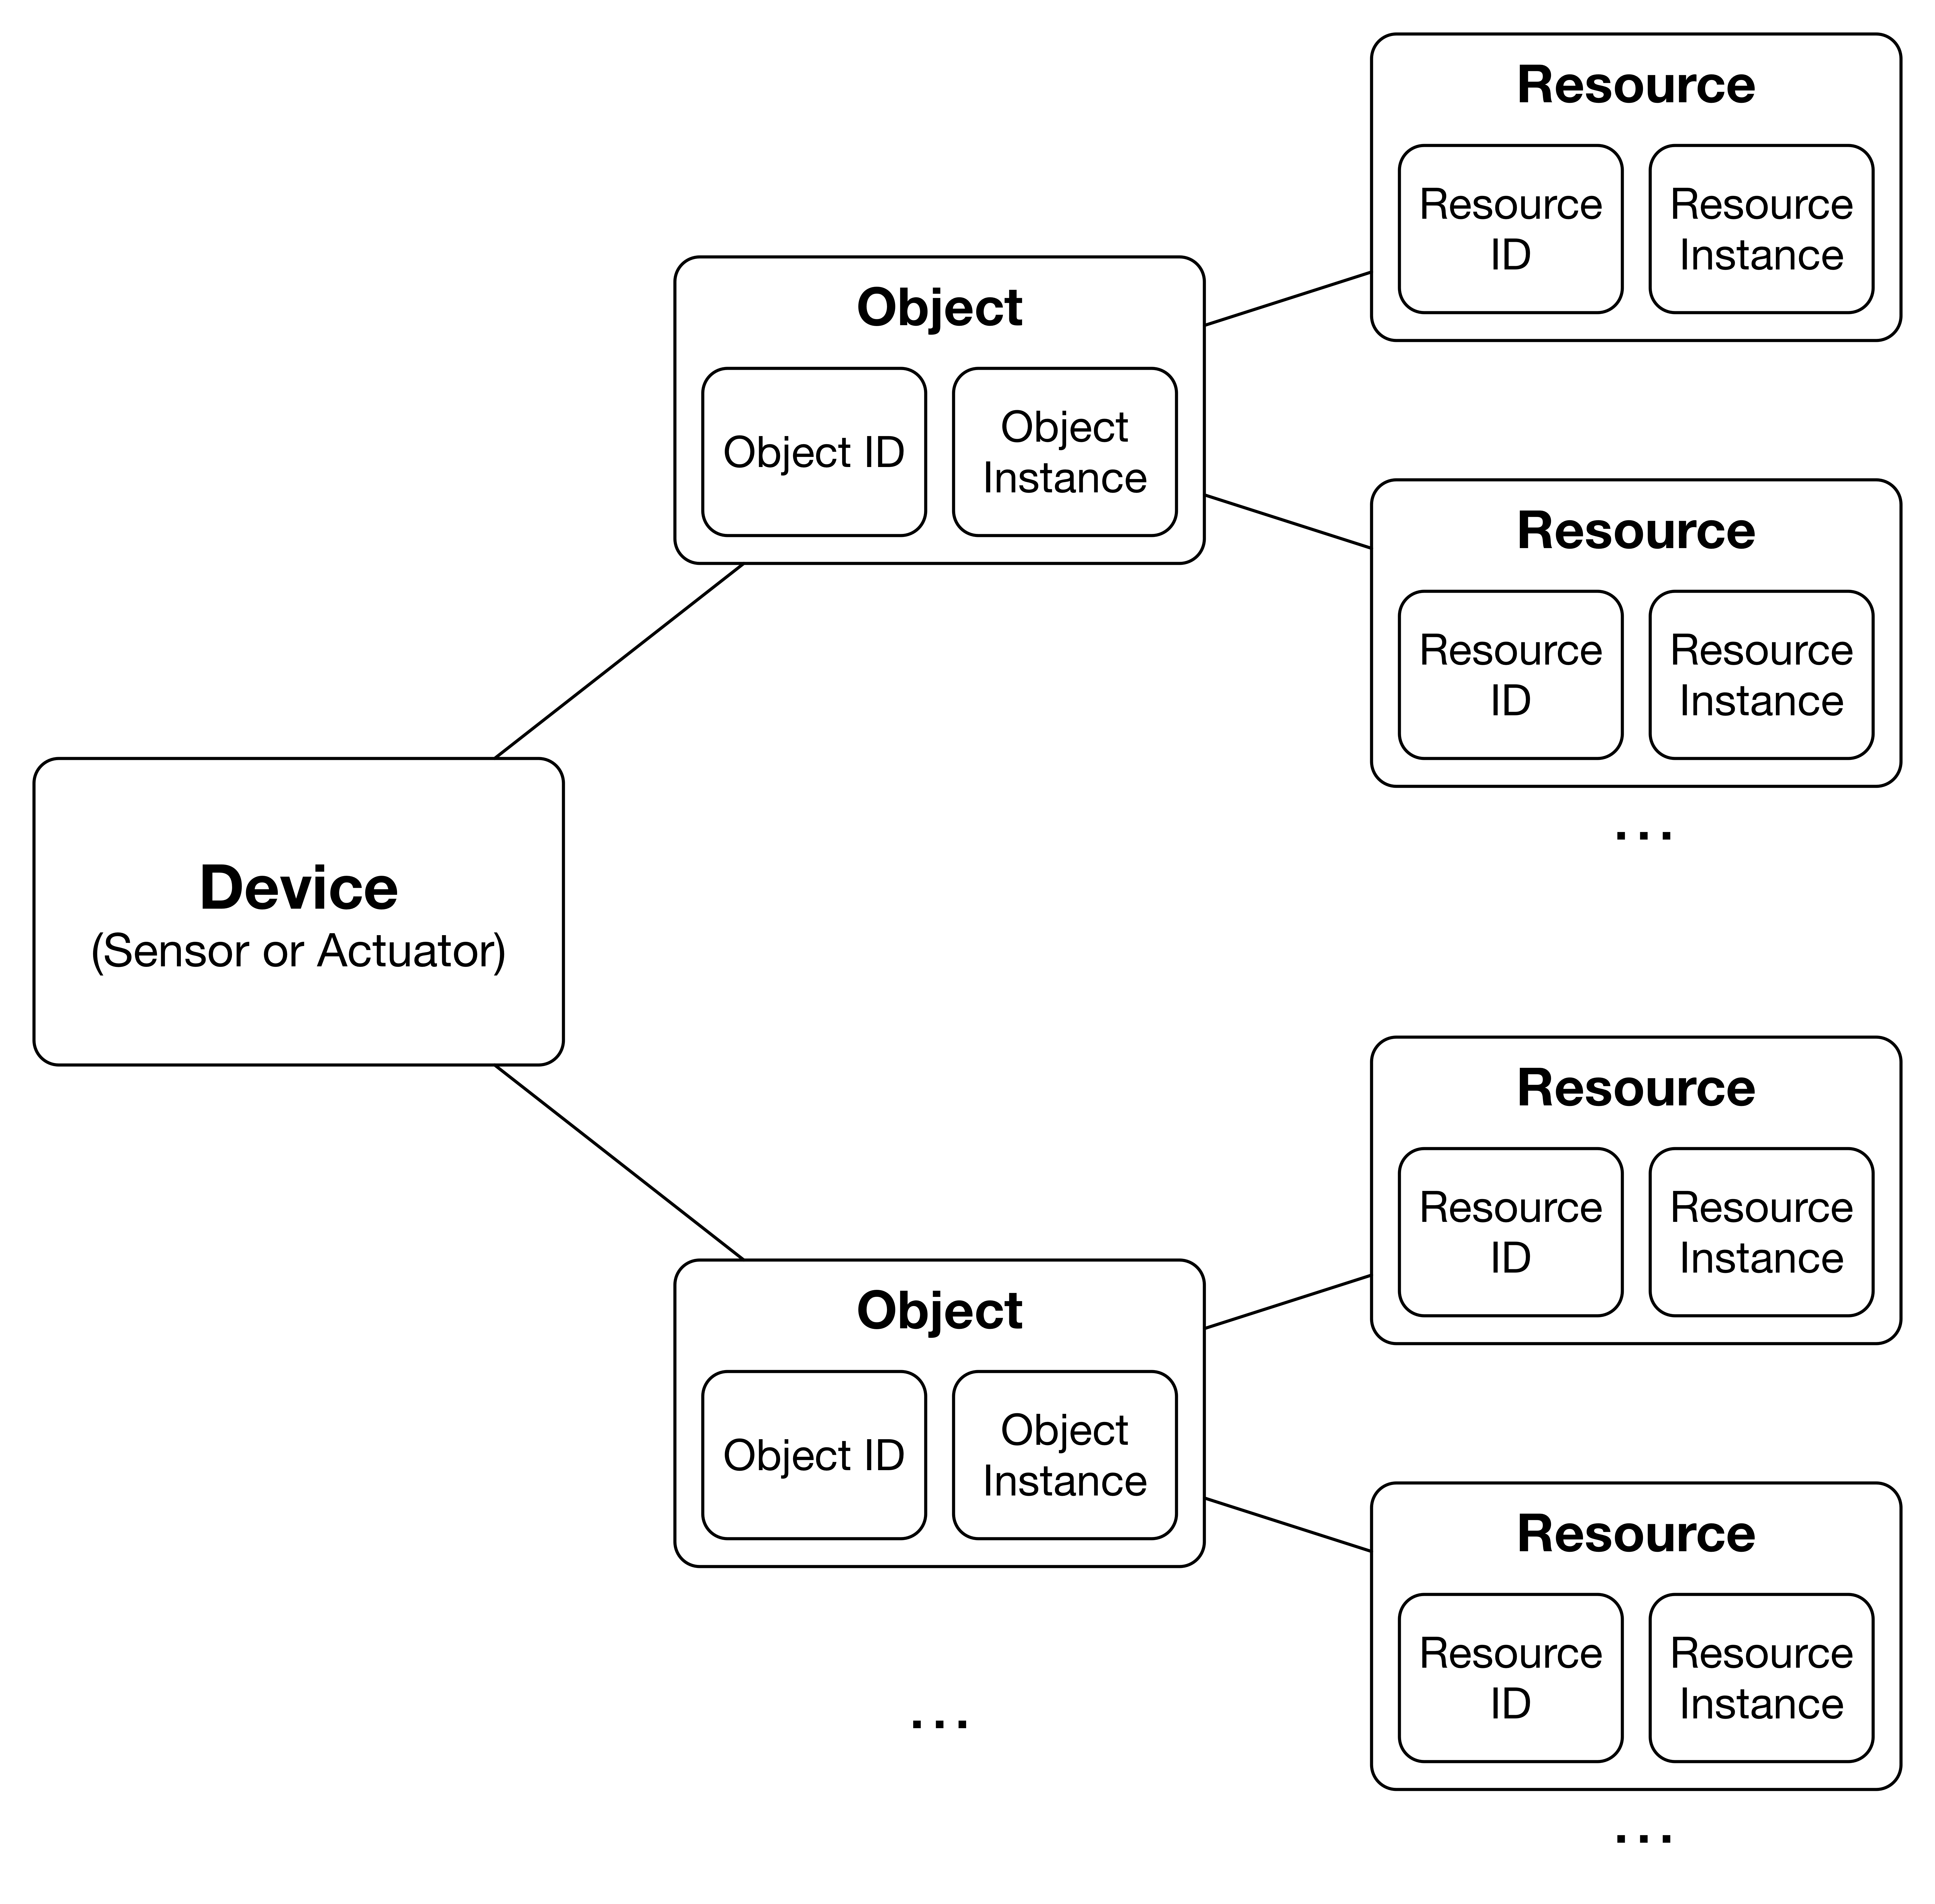
\includegraphics[width=0.9\textwidth]{figures/obj.png}
	\caption{Device objects representation}
	\label{fig:obj}
\end{figure}

In this representation, a device can have multiple objects (sensors and/or actuators), identified through an ID and an object instance. Per example, a device can have multiple sensing or actuating capabilities, each one of them identified with a different ID. A device with two motion sensors, will have two objects with the same ID but different object instances. 

Inside the representation of each object, the information is divided in resources. Resources represent the available features that each object provides, such as the available values that can be read or written, or the actions that can be triggered. As an example, an luminaire actuator object can have resources to read the current state of the luminaire, turn  on/off or dim the light to a certain value, each one of them represented with a different ID. The resource instance is used when, per example, when an actuator for aluminaire with two lamps offers the same resources for each lamp separately.

Using this representation, the properties of a device can me accessed using an Uniform Resource Identifier (URI) the following way: 


\begin{minted}[
frame=single
]{nginx}

.../Object_ID/Object_Instance/Resource_ID/Resource_Instance
	

\end{minted}
	
For instance, a device with a temperature sensor that offers the possibility of check the current state or check the minimum value measured by the sensor since it is ON, can be illustrated and accessed the following way:


\begin{figure}[H]
	\centering
	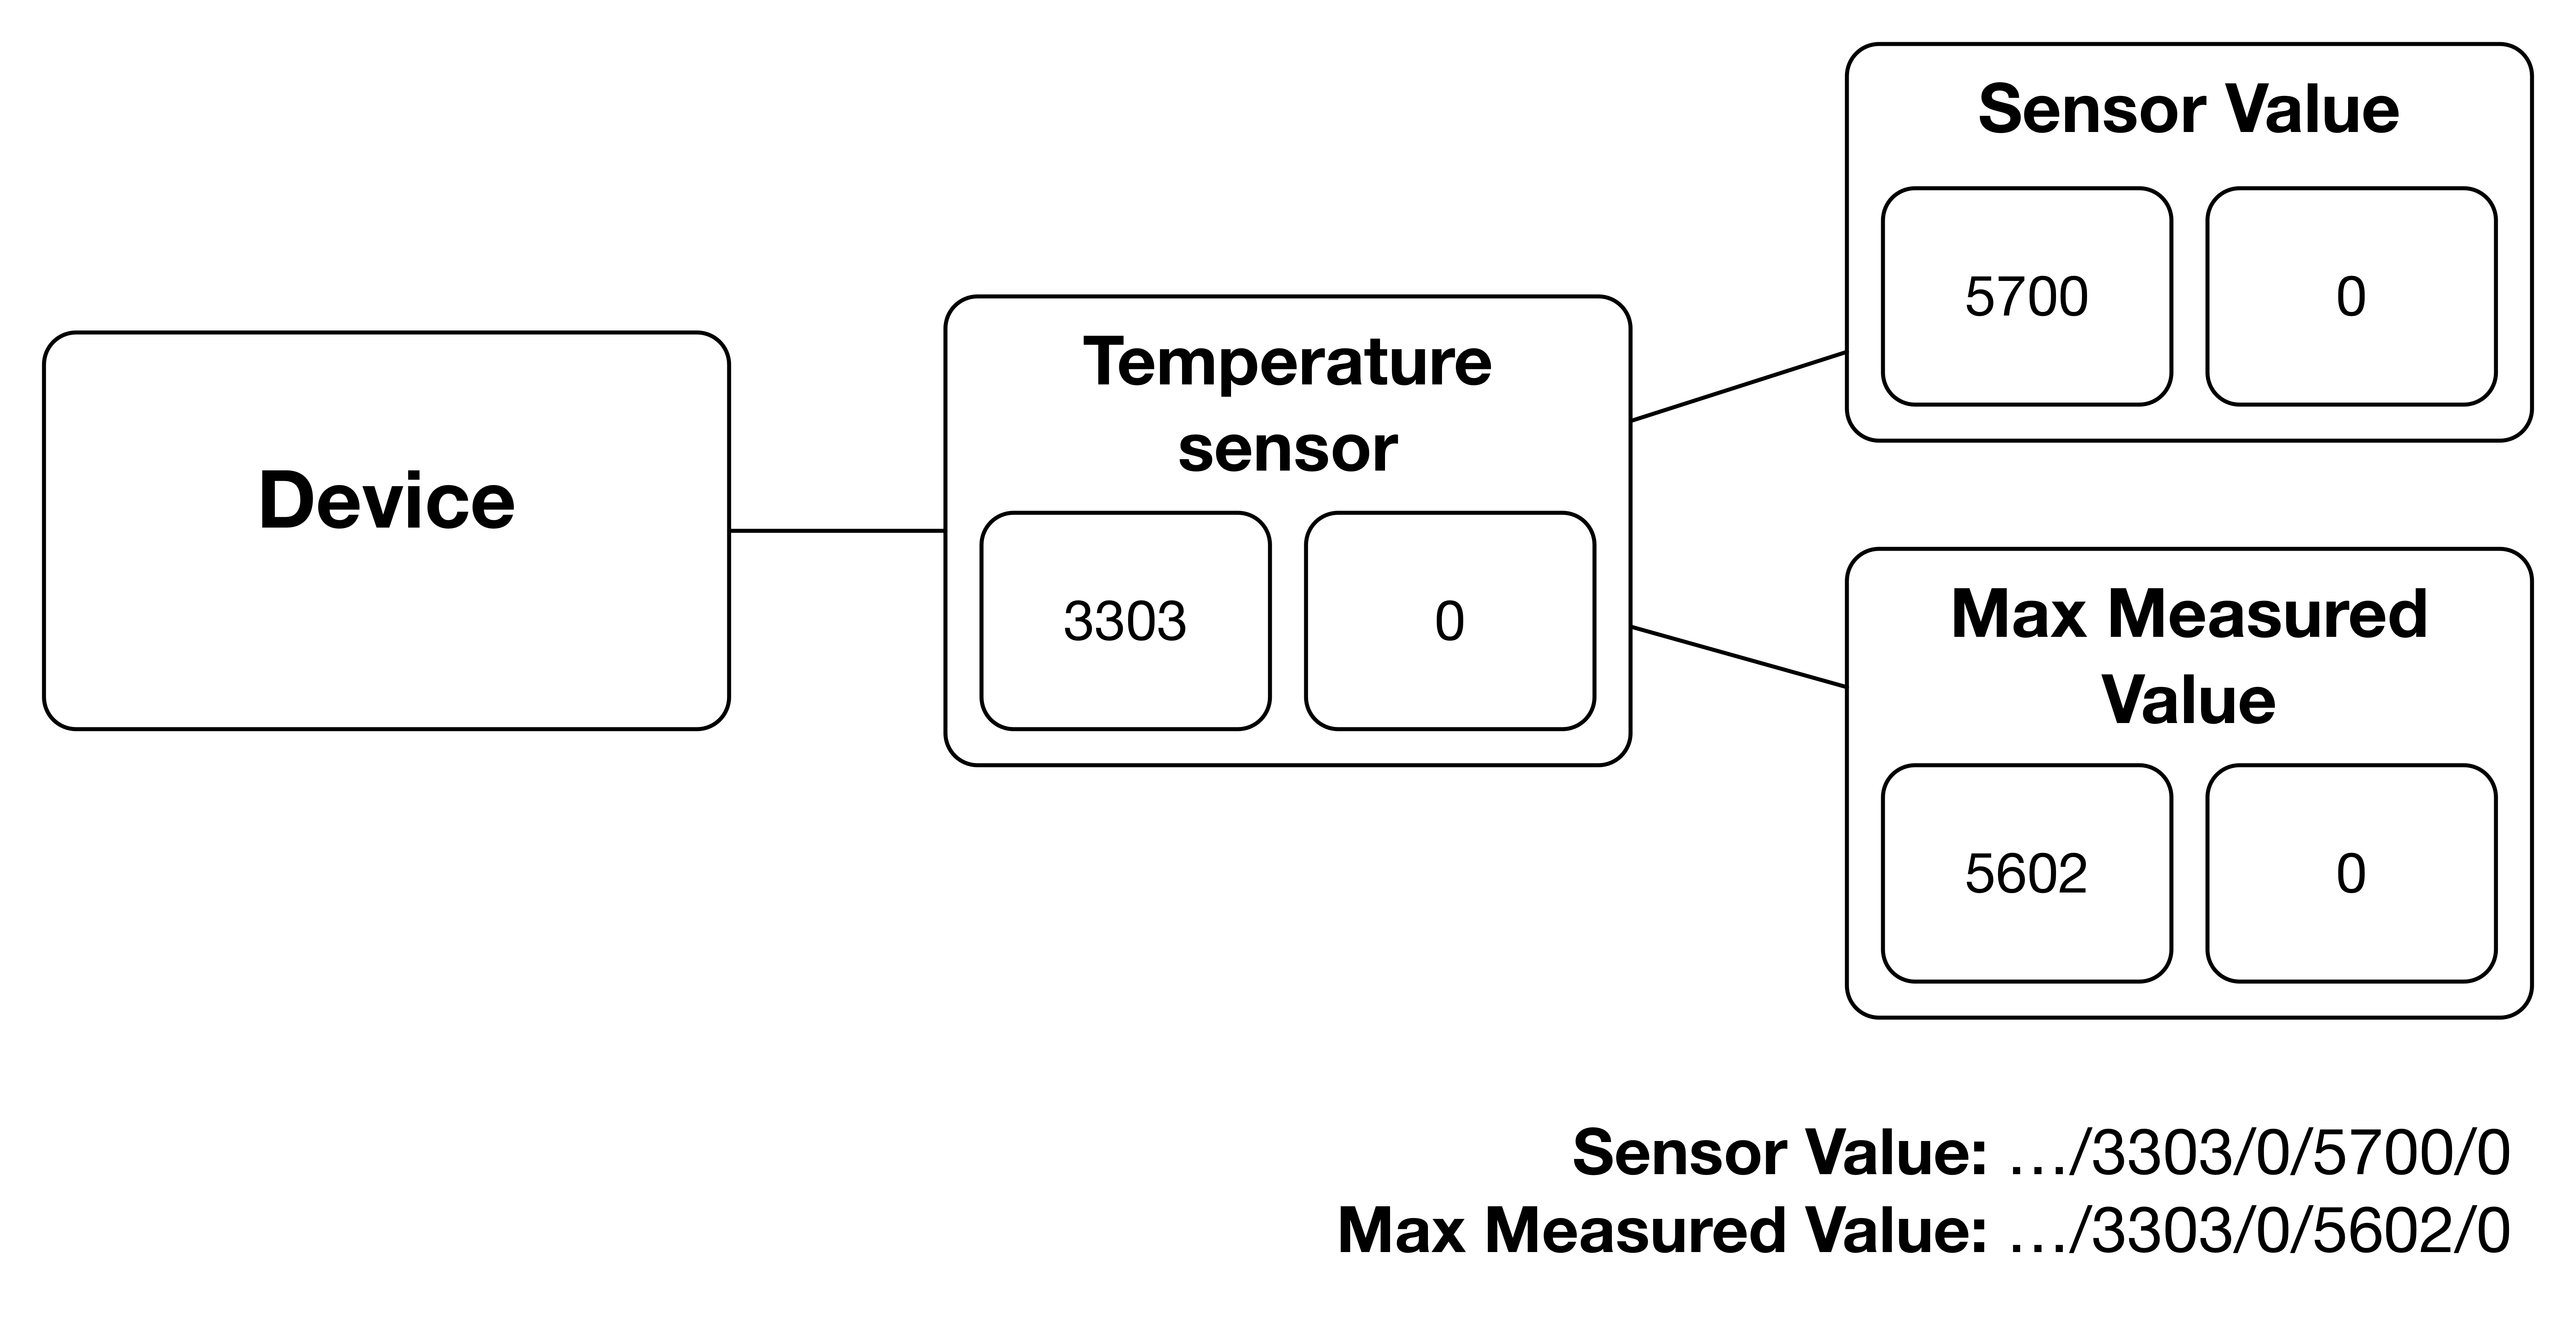
\includegraphics[width=0.9\textwidth]{figures/obj2.png}
	\caption{Access to a device resources.}
	\label{fig:obj2}
\end{figure}
	
Since the protocol used for this project was \ac{mqtt}, which allows to subscribe and publish messages in specific topics, this URI can be used in the topic to address each device resource. 

As stated before, due to the work done in other dissertation for this project, the message format to communicate with devices was chosen based on the event format supported by the WSO2 \ac{cep}, chosen as the \ac{cep} engine for this project. The format is represented in Snippet \ref{snippet:example}.

\begin{listing}[H]
\begin{minted}[
frame=single
]{json}

{
    "event": {
        "metaData": { 
            "attribute_1": ***,
            "attribute_2": ***,
            ...
        },
        "correlationData": {
            "attribute_1": ***,
            "attribute_2": ***,
            ...
        }, 
        "payloadData": {
            "attribute_1": ***, 
            "attribute_2": ***,
        }
    }
}


\end{minted}
\caption{Example of a simplified message for an event sent to a device.}
\label{snippet:example}
\end{listing}

This event messages are divided in three main logical sections: Payload Data, Correlation Data and Meta Data. Payload Data is the most important data to be transported, such as, the values that are sent to and from devices. The Correlation Data transports information that allows correlating events and lastly, the Meta Data is where other attributes that describe the event can be included. In Snippet \ref{snippet:todevice} is represented an example message of an event sent to a device.

\begin{listing}[H]
\begin{minted}[
frame=single
]{json}
{
    "event": {
        "metaData": {
            "operation":"set"
        }, 
        "payloadData": {
            "value": 15 
        }
    } 
}

\end{minted}
\caption{Example of a simplified message for an event sent to a device.}
\label{snippet:todevice}
\end{listing}

This message would set the value 15 on a device's resource if sent to the corresponding topic using the format presented above.

\section{Rules Standard}
\label{implementation:rules}


To obtain a fully autonomous system, rules must be designed in order to achieve it. In a previous dissertation of this project, a solution was designed to, instead of using directly the languages provided by each \ac{cep} engine which are difficult to map using a Graphical User Interface, a more extensible and pluggable solution was created. When a rule is made in the platform, a JSON is generated containing all the information needed to convert the rule to the desired engine, either the \ac{cep} engine or the Gateway engine, that will be addressed later.

In this solution, a Rule is divided in Actions, each one containing a Target and a Function. The Target specifies to where the output events, resulting from applying the rule, should be sent, while the Listeners inside the Function specify which input events trigger the rule. Also inside the Function, there can be present four types of modules to transform the event stream: Aggregators, Converters, Windows and Filters. Filters are used to select only events that pass a certain condition, otherwise the rule is not applied. Windows, allow to capture events in a given interval of time or occurrences following some criteria. This module is often used with Aggregators that perform aggregate calculations, such as summing the events or calculating averages. Lastly, the function of Converters is to make calculations with each event, for instance to preform unit conversions. There can also be used the Pattern and Sequence modules that, as the name says, are used to detect patterns or specific sequences of events.


In Snippet \ref{snippet:rule} is shown an example on an output JSON of a rule with a single action. As can be observed, a rule can be constituted by sub rules. Each sub rule within a Rule has the same Function but different Targets and Listeners. In this particular case, the rule has a function called "setif\_value\_percent" with two different types of Listeners, a "listen\_boolean" and a "listen\_value". The first is used to listen to boolean values (which in this case are the motion sensor state) and the last to listen to float values (luminance sensors, in this case). The boolean data is read for a 6 seconds time window and aggregated with the “any” Aggregator which detects if there was any motion in the last 6 seconds. The data containing the luminance values, is aggregated with an average over the last 5 events, and converted using the converter “lux\_to\_percent”. Therefore, the function sends to the target an event with the 100\% calculated percentage if a motion is detected in the last 6 seconds, and 50\% otherwise. 


\begin{listing}[H]
	\begin{minted}[
	frame=single
	]{json}
{
    "name": "Labs Lights",
    "subrules": [{
        "actions": [{
            "target": {
                "type": "mqtt",
                "topic": "/SM/out_events/IT2/Floor_1/Lab/1.10/1/*/3302/*/5851/*",
                "value_type": "int"
            },
            "function": {
                "name": "setif_value_percent",
                "listen_boolean": {
                    "type": "single",
                    "listeners": [{
                        "type": "mqtt",
                        "topic": "/SM/IT2/Floor_1/Lab/1.10/1/+/3302/+/5500/+",
                        "value_type": "int"
                    }],
                    "window": {
                        "type": "time",
                        "units": "seconds",
                        "value": 6
                    },
                    "aggregator": {
                        "type": "any"
                    }
                },
                "listen_value": {
                    "type": "single",
                    "listeners": [{
                        "type": "mqtt",
                        "topic": "/SM/IT2/Floor_1/Lab/1.10/1/+/3301/+/5700/+",
                        "value_type": "float"
                    }],
                    "window": {
                        "type": "length",
                        "value": 5
                    },
                    "aggregator": {
                        "type": "avg"
                    },
                    "converter": {
                        "type": "lux_to_percentage",
                        "value": 50
                    }
                },
                "percent_if_true": 100,
                "percent_if_false": 50
            }
        }]
    }]
}
	\end{minted}
	\caption{Example of a JSON rule outputted be the Building Manager platform.}
	\label{snippet:rule}
\end{listing}



	
\section{Architecture}
\label{implementation:architecture}
Taking into consideration the objectives and adopted technologies addressed in chapters \ref{implementation:objectives} and \ref{implementation:technologies}, the implemented architecture is represented in Figure \ref{fig:arch2}. Comparing this architecture to the one presented in Figure \ref{fig:arch}, it is clear the use of MQTT as the main communication protocol, the removal of the User Management component, since it was not in the scope for this dissertation, and as far as the \ac{cep} engine and the Building Manager concerns, those components were already implemented, as stated before. The BLE Adapter which is part of the gateway was also already implemented. Lastly, the MQTT broker used in this implementation was Mosquitto\footnote{https://mosquitto.org/}, which is a lightweight broker suited for \ac{iot} environments which implements the latest versions on MQTT protocol . 

For the scope of this dissertation, the focus was the implementation of a Gateway with automation capabilities, and also a Gateway Manager to handle not only the rule and device distribution between the available gateways, but also to handling fails in order to maintain the system working even in emergency states.


\begin{figure}[H]
	\centering
	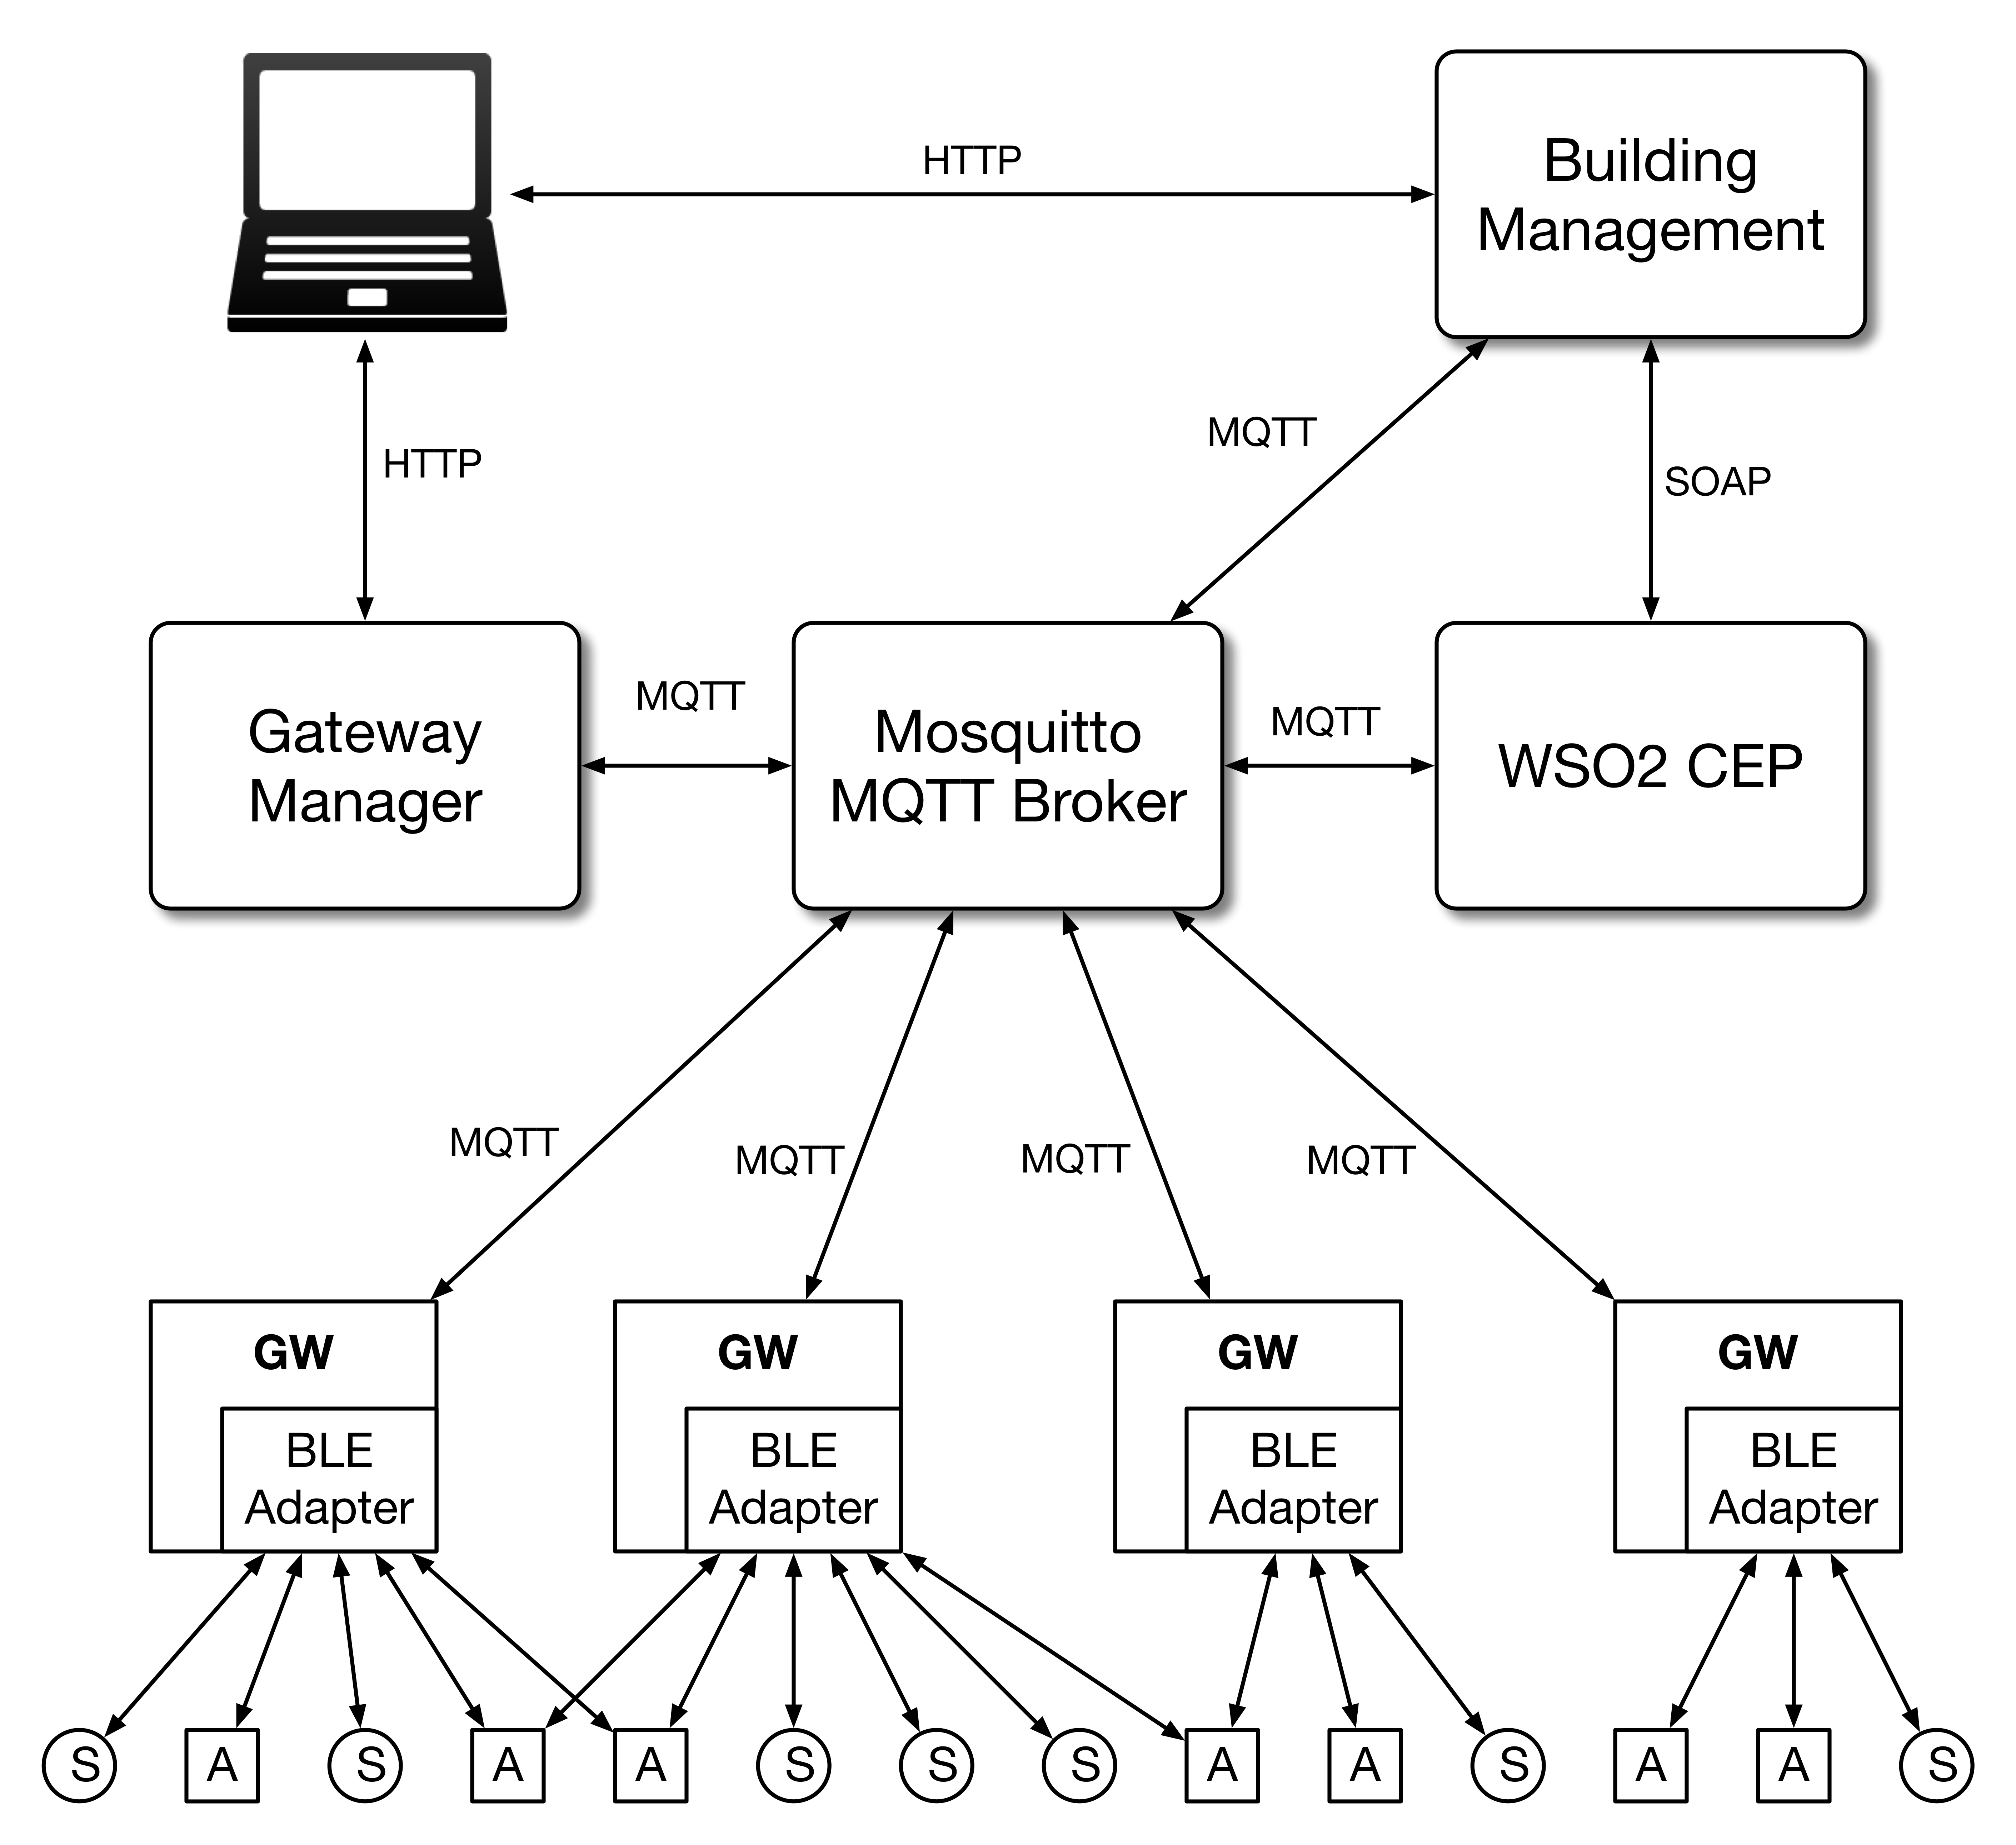
\includegraphics[width=0.8\textwidth]{figures/architecture3.png}
	\caption{Implementation Architecture}
	\label{fig:arch2}
\end{figure}

\subsection{Gateway Manager}
\label{arch:gm}

This section will describe how the Gateway Manager fits in the fulfilment of the requirements and objectives proposed for this project, and also how its features were thought and implemented. 


This component was programmed using Python 3\footnote{https://docs.python.org/3/} and since MQTT was the chosen protocol to communicate with other nodes, the Eclipse Paho MQTT Python client\footnote{https://pypi.python.org/pypi/paho-mqtt/1.3.0} library was used. This client enables the application to connect to a MQTT broker in order to publish messages and subscribe to topics. Bellow will be described the most important features implemented for this component.


\begin{Paragraph}{Rule Parsing and Distribution}
	
One of the Gateway's Manager roles is to receive rules, developed in the existing Building Manager platform. As addressed before, a rule is represented in JSON format, and when the rule is set to be deployed in the gateways automation engine, the Gateway Manager parses it in order to divide the rule in sub rules and distribute them among the available gateways. To keep track of which rules are deployed where, and to which rule's different targets and listeners correspond, the \ac{gm} attributes a unique ID to each rule and stores, in data structures, the topics(from input and output events) used in each rule and to which rule IDs they correspond, since different rules can have the same targets and/or listeners. This data structures will be important to implement the fail handling measures, which will be addressed later. Bellow, in Figure \ref{fig:parser_struct}, can be seen the data structure used to store this information.

\begin{figure}[H]
	\centering
	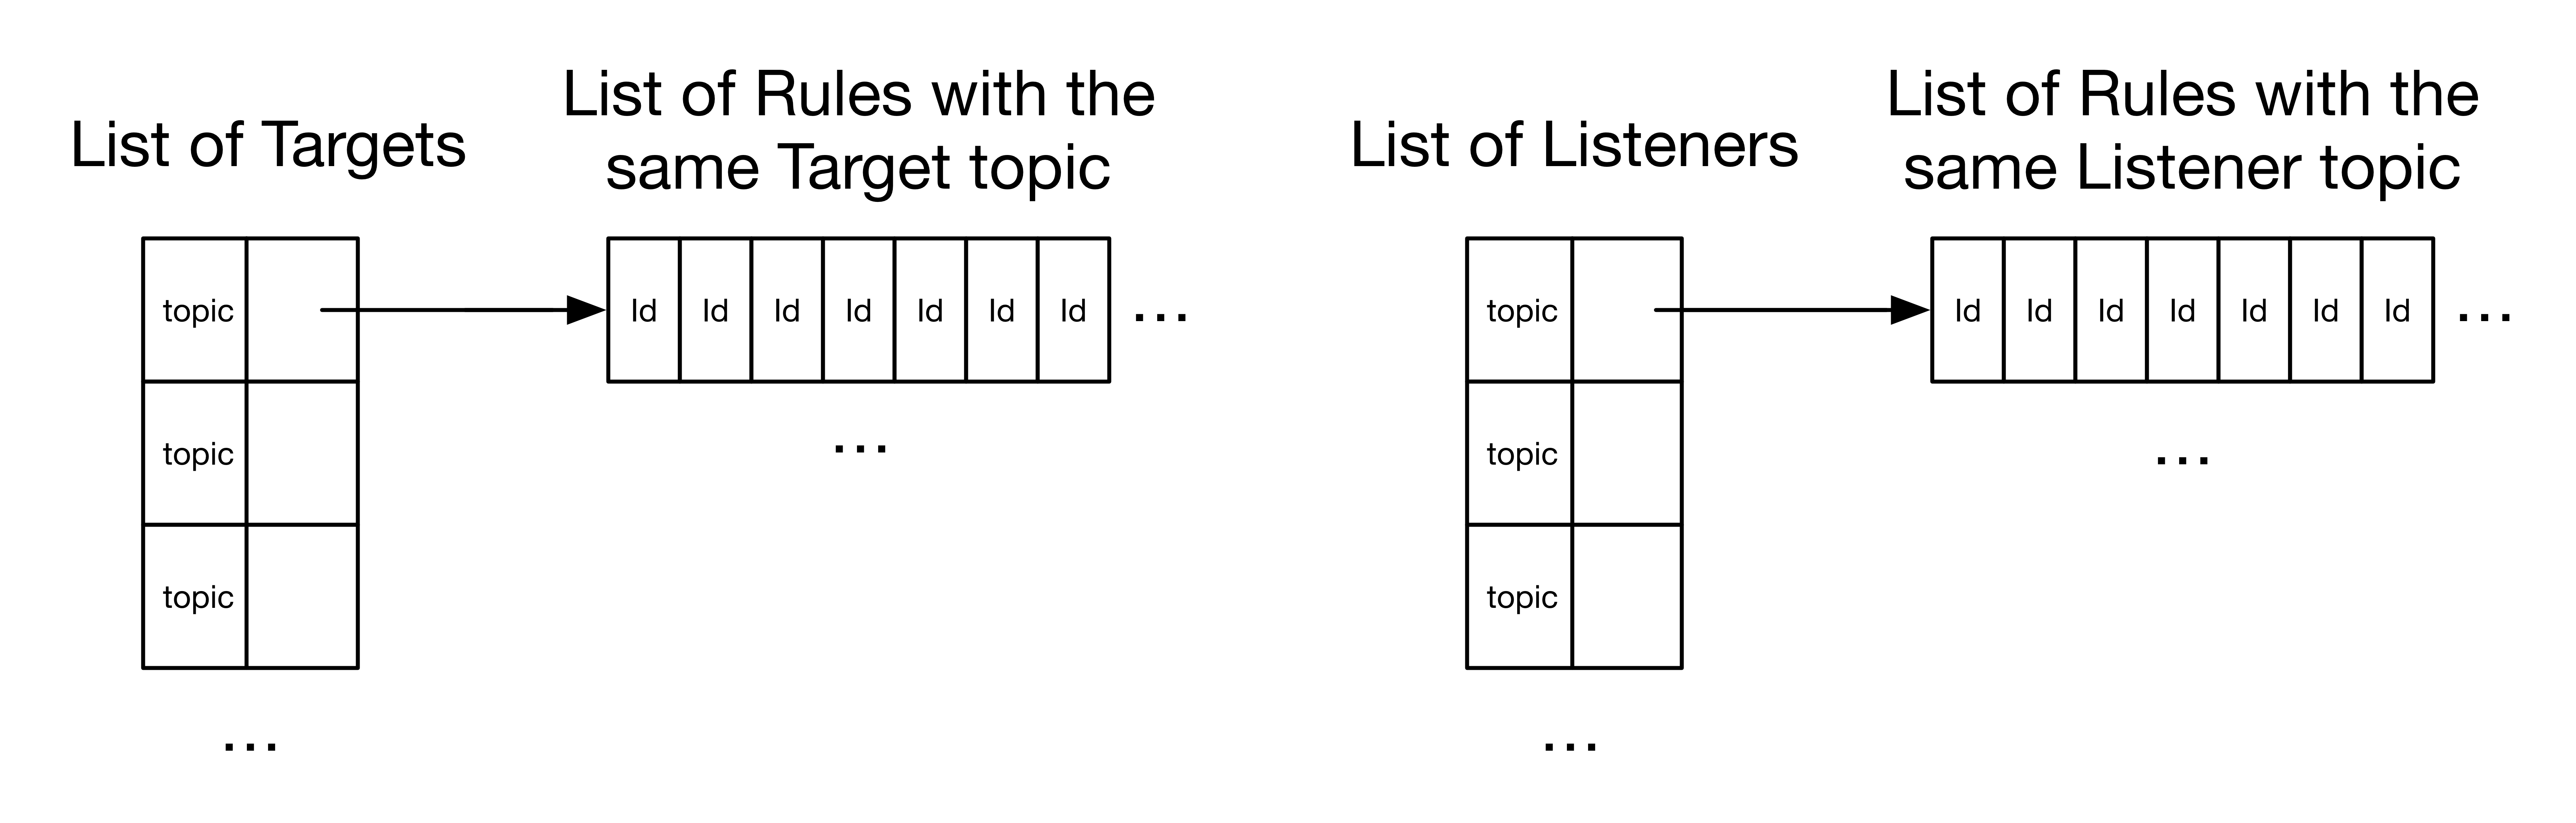
\includegraphics[width=0.9\textwidth]{figures/parser_struct.png}
	\caption{Data structures used to store Targets and Listeners and to which Rule IDs they correspond.}
	\label{fig:parser_struct}
\end{figure}

After the rule is parsed, the \ac{gm} distribute the sub rules to the available gateways using a round-robin method, in order to maintain a equal number or deployed rules among gateways. Bellow, in Figure \ref{fig:addrule} can be observed an interaction diagram of the communication needed to add a new rule to the Gateway Manager and a Subrule to a Gateway, using MQTT.

\begin{figure}[H]
	\centering
	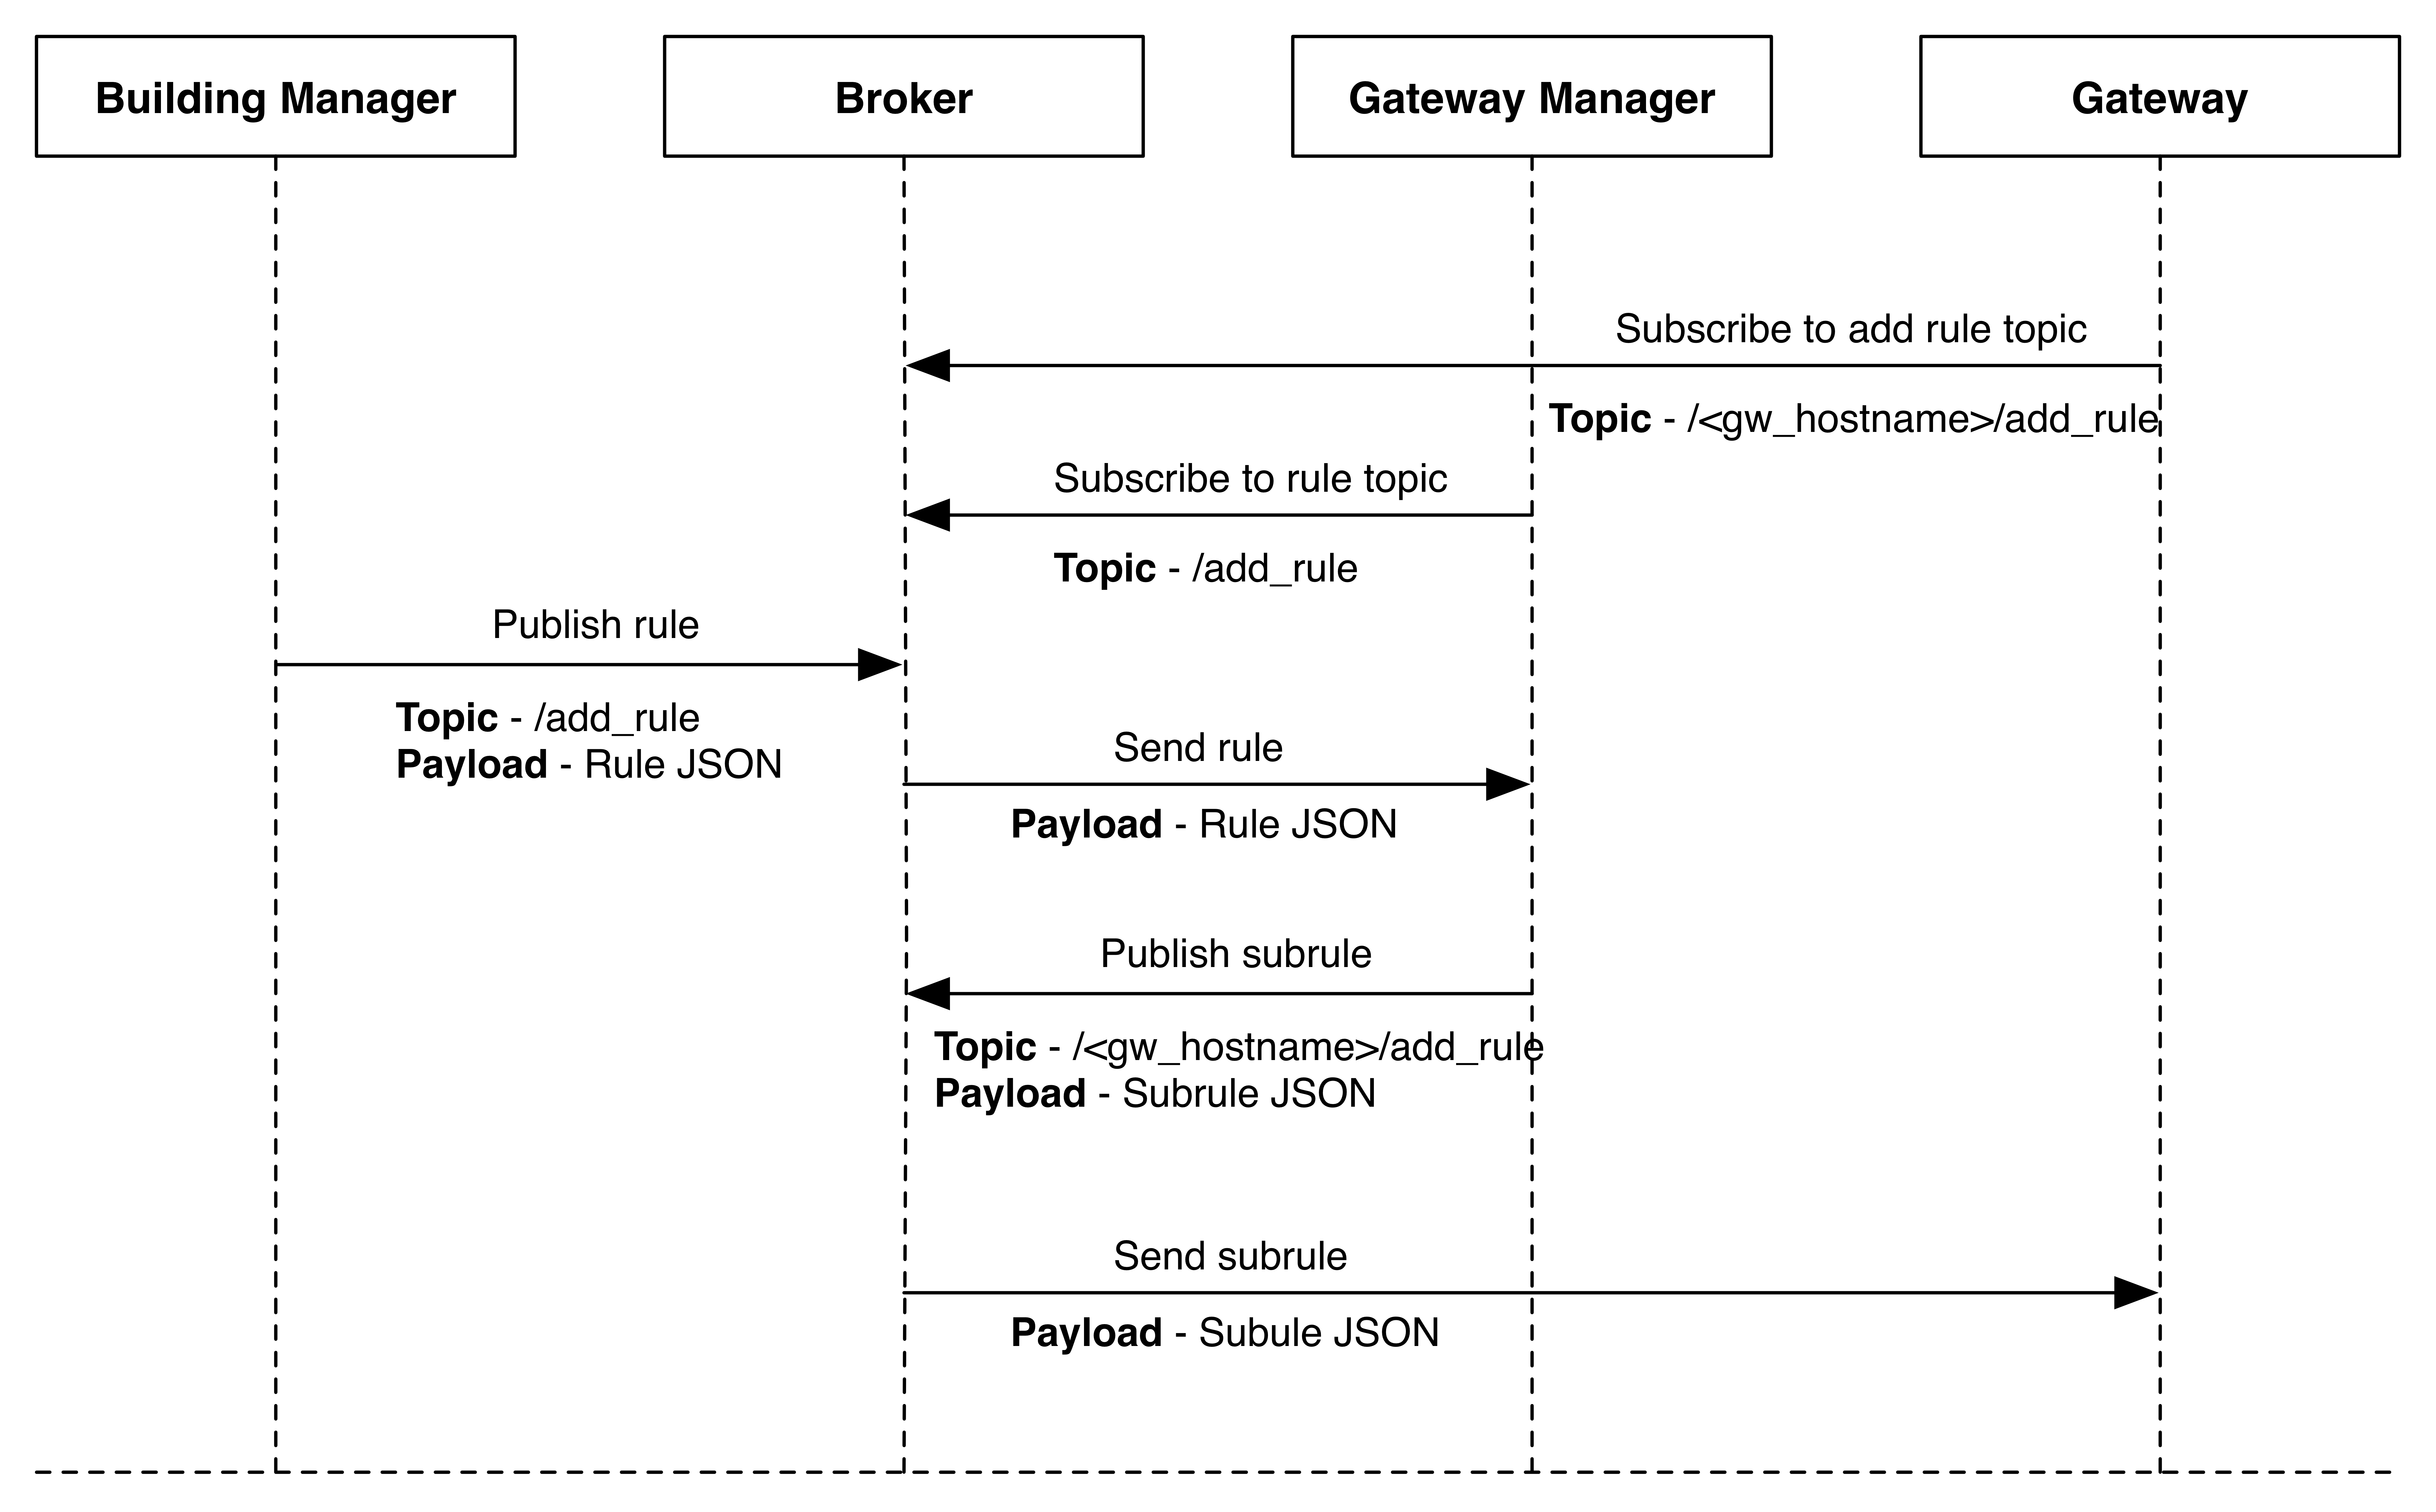
\includegraphics[width=0.9\textwidth]{figures/addrule.png}
	\caption{Interaction diagram of adding a new rule to the Gateway Manager and a Subrule to a Gateway.}
	\label{fig:addrule}
\end{figure}

\end{Paragraph}

\begin{Paragraph}{System Awareness}

The \ac{gm}, being the unit that will impose the fail handling measures, needs to be aware of each component and each gateway state. In order to do that, each component has to send a periodic heart beat message to the central broker, using the "/heart\_beat" topic, which is subscribed by the \ac{gm}. The \ac{gm} then checks periodically if every component sent the heart\_beat. If a component fails and it is not able to send the heart\_beat, after a programmable timeout, the \ac{gm} begins the implementation of failing handling measures.

\end{Paragraph}

\begin{Paragraph}{Devices Configuration}

When new a gateway is connected to the system, it sends a message to the \ac{gm}, informing which devices it is able to connect and then, with this information, the \ac{gm} balances the available devices among the gateways. To explain further, when two gateways are able to connect to the same devices, the \ac{gm} balances that devices among the two in order to maintain a equal number of devices in each one. Also, it stores for each device, the gateways that are able to connect to it. This allows that when a gateway fails, the \ac{gm} has all the information needed to inform the gateways that are able to connected to the lost devices, to take control of those devices.

\end{Paragraph}

\begin{Paragraph}{Building Manager Dashboard}

In order to visualize the state of the gateways present in the system, a dashboard was created, using Python3 web framework Flask\footnote{http://flask.pocoo.org/}. In Figure \ref{fig:main_gm} is shown the main page of this dashboard.

\begin{figure}[H]
	\centering
	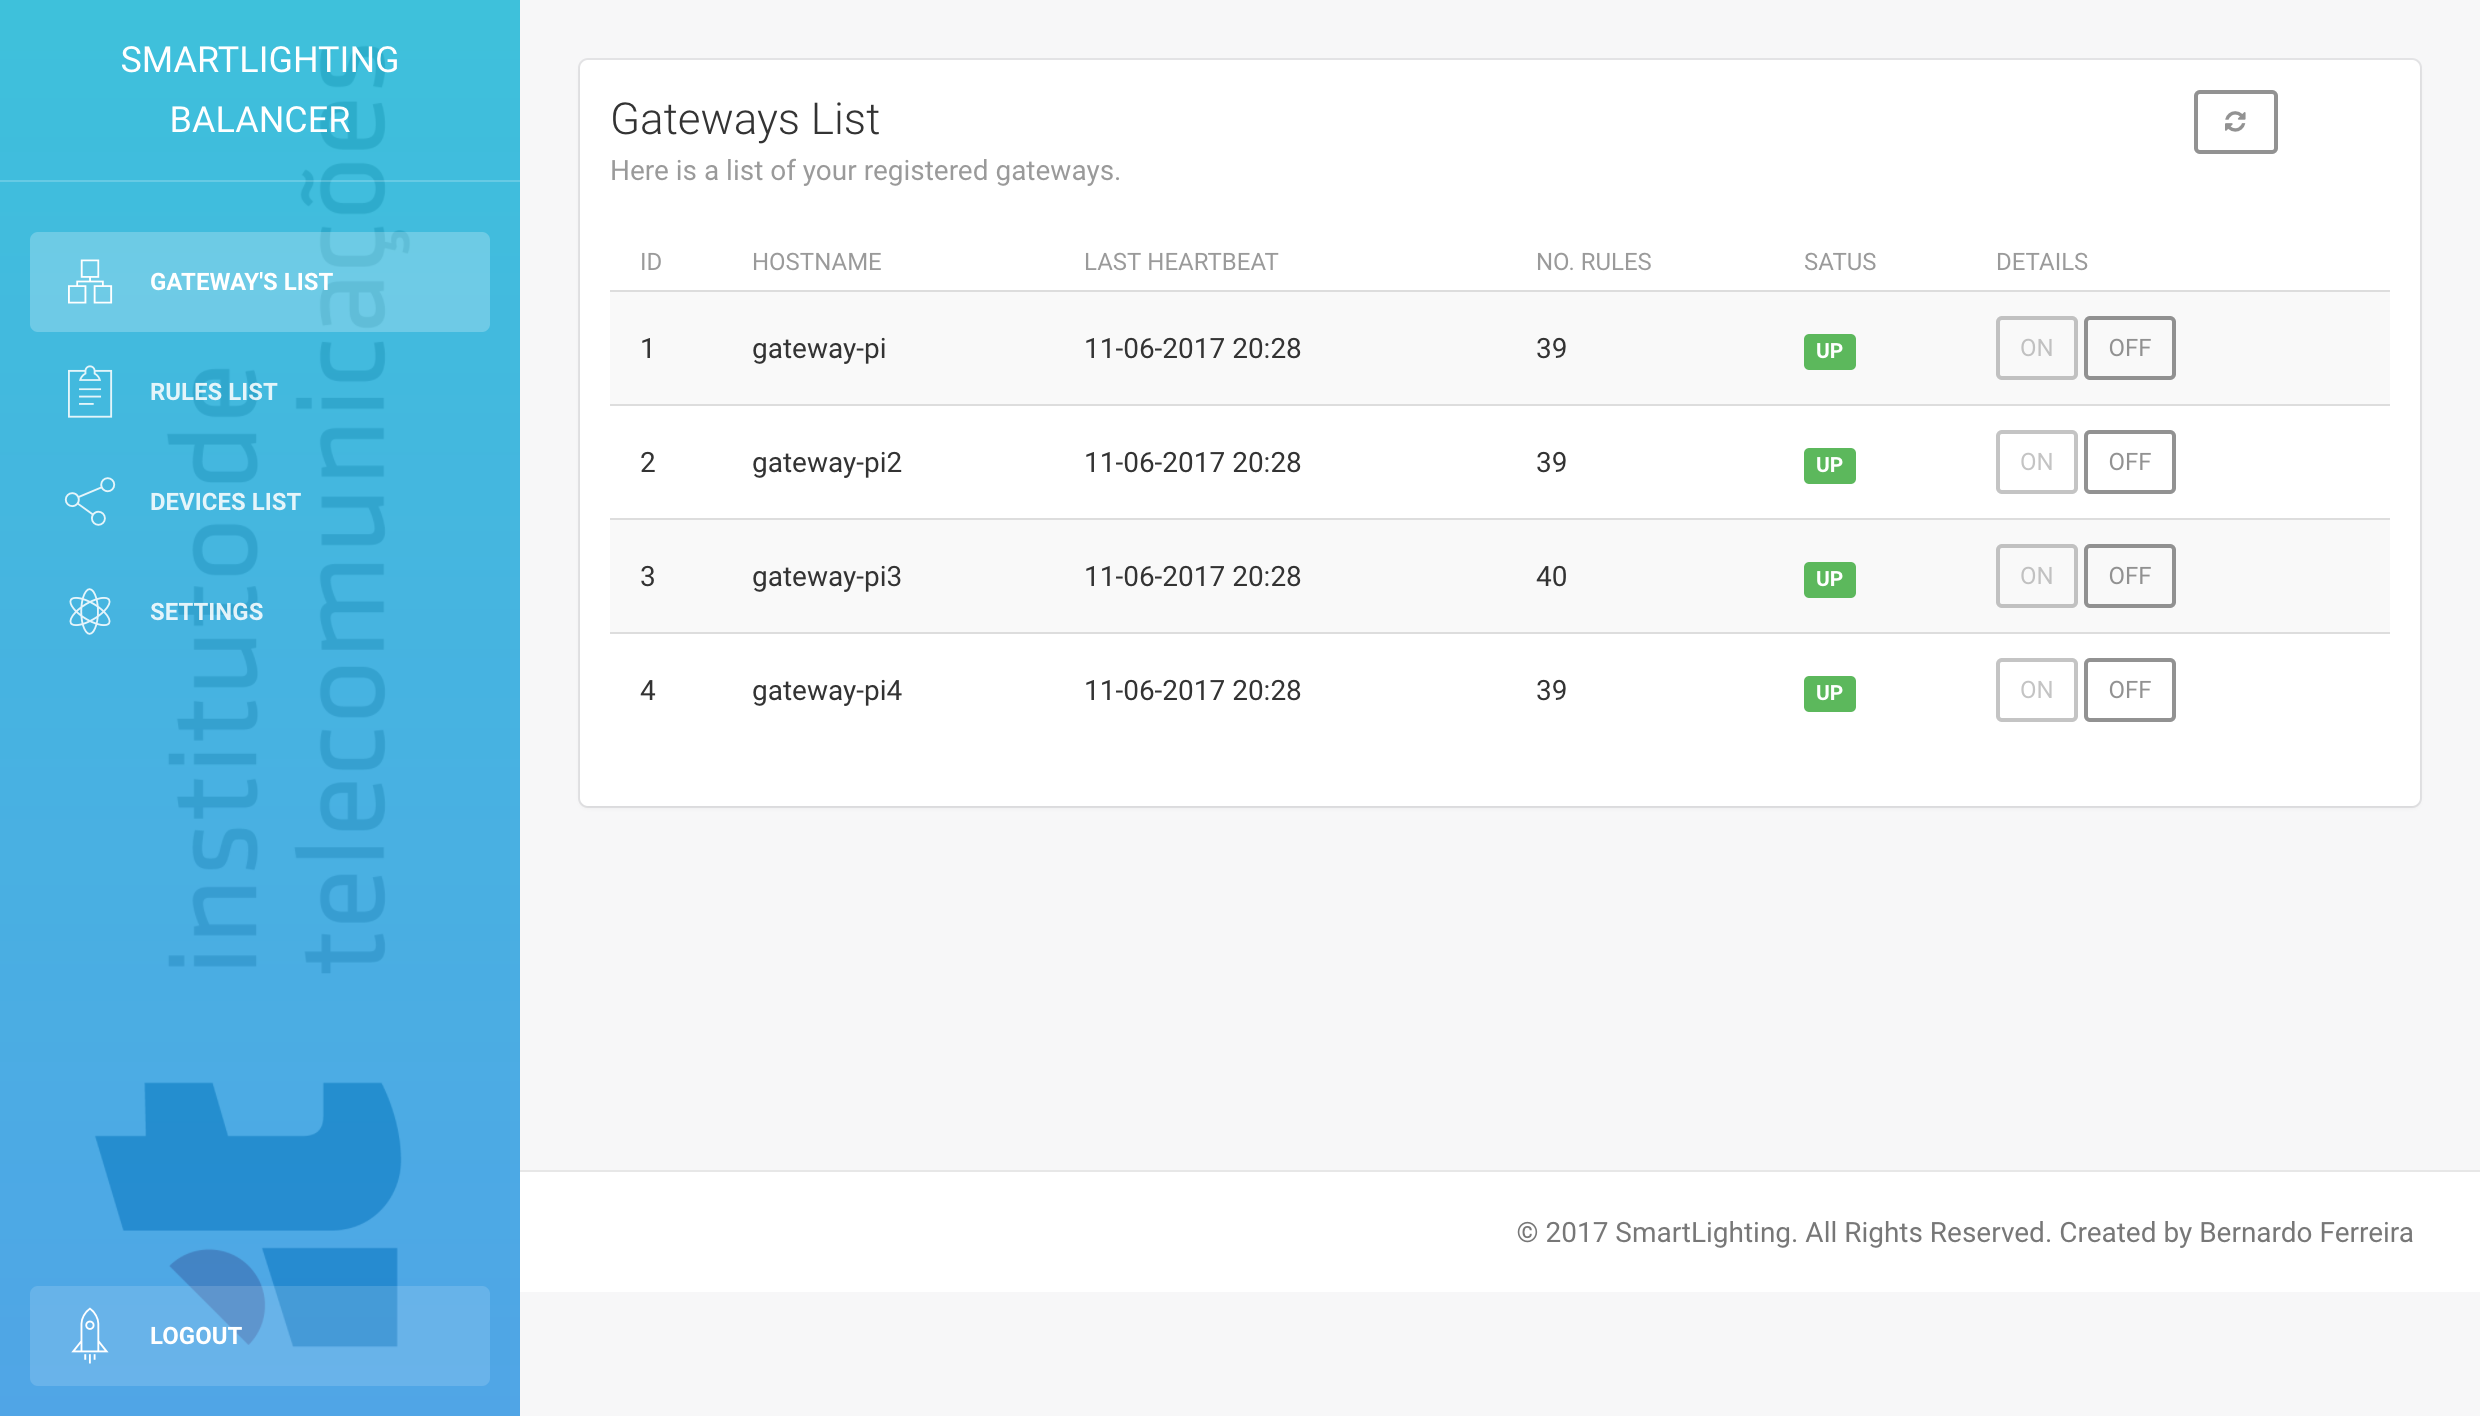
\includegraphics[width=0.9\textwidth]{figures/main_gm.png}
	\caption{Screenshot of the Gateway Manager dashbord main page.}
	\label{fig:main_gm}
\end{figure}

As can be observed, this dashboard allows to check several information about the gateways, such as, the hostnames, the time of the last heart beat received, the number of devices connected, and has also a feature to turn on/off a gateway if pleased. Also, it has not only the the list of rules and in which gateway they are being deployed, but also a list of devices and the corresponding gateway.


\end{Paragraph}

\begin{Paragraph}{Gateway Failure Handling}
	
Since Gateways are the components that communicate directly with devices, a gateway failure could have a huge impact for the building. For that reason, one of the most important features of the \ac{gm} is to detect that a gateway fails and, as addressed before, inform other gateways within the range of the lost devices to assume control. Also, the rules that were present in the failing gateway, should also be sent to other gateways to be deployed. Bellow in Figure \ref{fig:gwdown}, it is represented the interaction diagram of the processes that occur when a gateway fails. 

\begin{figure}[H]
	\centering
	\includegraphics[width=0.9\textwidth]{figures/gwdown.png}
	\caption{Interaction diagram of the procedures when a gateway fails.}
	\label{fig:gwdown}
\end{figure}
	
As can be observed, since the \ac{gm} has all the information, regarding which gateways have access to which devices, it can easily distribute the lost devices among the gateways that can communicate with them. Also, the rules that were deployed in the lost gateway are distributed through the available gateways using, again, a "round-robin" method in order to balance the number of rules in each gateway.  

\end{Paragraph}

\subsection{Gateway}
\label{arch:gw}

This section will describe how the Gateway proposed features and its requirements were implemented. Since this project aims to create a smart environment in buildings, the amount of gateways needed to cover the whole network of devices may vary depending on the building size. Most solutions in the \ac{bas} systems rely on expensive gateways which can be a downside for stakeholders. The solution is to create a gateway software that are able to work in a microcontroller or in a small and cheap \ac{soc} like a Raspberry Pi\footnote{https://www.raspberrypi.org/} or a Nano Pi\footnote{http://www.nanopi.org/}. With this in mind, the programming language proposed used in the deployment of this software was MicroPython\footnote{https://micropython.org/}. MicroPython is an open source Python programming language interpretor that runs on small embedded development boards \cite{micro2} and, although being full packed with advanced features, it is compact enough run within just 256k of code space and 16k of RAM \cite{micro}. For this reasons, MicroPython was chosen to allow more flexibility when choosing gateway's hardware.

To allow the communication between gateways and with the \ac{gm}, a Mosquitto lightweight MQTT broker was also deployed in each gateway. Also, since the IP addresses of the several components, which are needed to communicate with each others, can change due to network problems, it was deployed in each node of the system an Avahi deamon\footnote{https://www.avahi.org/}, enabling that each component could be reached by just its hostname, which never changes for each machine.

Bellow, will be addressed the implemented features on Gateway's software.

\begin{Paragraph}{Devices Configuration and Management}

When a gateway is deployed, it needs to send, to the \ac{gm} a list of devices within its range and the resources that each device has. Later, the \ac{gm}, responds with a list of which devices should be controlled by the gateway and in which topics should gateways publish events generated by the devices. Also, gateways receive information concerning to which topics they must subscribe in the central broker. To explain further, gateways need to know in which topic to publish events, generated by each device, in the central broker. Also, after those events being processed in the CEP Engine, gateways need to be subscribed to the output event topics that concern the devices it controls, in order to receive the automation actions. Bellow, in Figure \ref{fig:newdevice}, is represented the interaction diagram of the communications needed to configure a new device. 


\begin{figure}[H]
	\centering
	\includegraphics[width=0.9\textwidth]{figures/newdevice.png}
	\caption{Interaction diagram of a new device configuration.}
	\label{fig:newdevice}
\end{figure}


	
\end{Paragraph}

\begin{Paragraph}{Rule Parser}

The \ac{gm}, as addressed before, parse the received rules and give an unique ID to each subrule. Then, when balancing the rules among the available gateways, it sends a JSON with the subrule and the given ID. When a sub rule is received in a gateway, it must be deconstructed in order to the automation engine know which events trigger it and what actions must be performed. In Figure \ref{fig:parse} it is represented a flow diagram explaining the process of parsing a rule. As addressed before, each subrule can either have a Set Value or a Set Percent Function. In Set Value Functions, there is only one action to be parsed, however, in Set Percent Functions, there are two actions to be considered, a Listen\_value and a Listen\_boolean action. For each action, the parser checks the existence of the modules addressed before, i.e. Windows, Aggregators, Filters and Converters, and creates an object for each one of them, containing its informations. An Action object is then created, containing an unique ID and a reference for the modules objects. In the end, the parser saves in a data structure, the information regarding the rule in the following way: \textit{Rules[Listeners] = [ActionsID]}, where, Rules is a list of MQTT topics, of the different listeners parsed, and each one of them has a list of ActionsIDs with the same Listener. This was implemented this way so that when an event is received, it is only needed to search for the corresponding Listener topic, in the data structure, to know which actions must be triggered. 


\begin{figure}[H]
	\centering
	\includegraphics[width=0.8\textwidth]{figures/parseRule.png}
	\caption{Rule parser flow diagram}
	\label{fig:parse}
\end{figure}

\end{Paragraph}

\begin{Paragraph}{Gateway Automation Engine}

The \acf{gae}, as stated before, will only work in emergency states, either if the central broker or the \ac{cep} Engine are down. When this happens, the gateways will start to receive in events in its internal broker. As mentioned earlier, when an event arrives to a gateway, first it must discover the Actions that need to be triggered so that the event can be processed. The \ac{gae} was designed to implement the modules present in Table \ref{module-table}.
 
\begin{table}[H]

	\resizebox{\textwidth}{!}{\begin{tabular}{|c|c|l|}
		\hline
		\textbf{Type}               & \textbf{Module}       & \textbf{Description}                                                                                                                                            \\ \hline
		Listener                    & MQTT                  & MQTT topic to receive events                                                                                                                                     \\ \hline
		Target                      & MQTT                  & MQTT topic to send events                                                                                                                                        \\ \hline
		\multirow{2}{*}{Function}   & Set Value             & Set the value received from input streams to the output streams                                                                                                 \\ \cline{2-3} 
		& Set Percent           & \begin{tabular}[c]{@{}l@{}}Set a percentage of a value from input streams to the output\\ streams, based on boolean data from another input stream\end{tabular} \\ \hline
		\multirow{6}{*}{Filter}     & Equal                 & Filter events with the value equal to a given value                                                                                                             \\ \cline{2-3} 
		& Not Equal             & Filter events with the value different than a given value                                                                                                       \\ \cline{2-3} 
		& Greater Than          & Filter events with the value greater than a given value                                                                                                         \\ \cline{2-3} 
		& Less Than             & Filter events with the value less than a given value                                                                                                            \\ \cline{2-3} 
		& Greater or Equal Than & Filter events with the value greater or equal to a given value                                                                                                  \\ \cline{2-3} 
		& Less or Equal Than    & Filter events with the value less or equal to a given value                                                                                                     \\ \hline
		\multirow{2}{*}{Window}     & Time Window           & Capture events in a predefined time                                                                                                                             \\ \cline{2-3} 
		& Length Window         & Capture a predefined number of events                                                                                                                           \\ \hline
		\multirow{3}{*}{Aggregator} & Average               & Calculate the average value of all the events in a window                                                                                                       \\ \cline{2-3} 
		& Any                   & Returns 1 if any of the values in the window is greater than 0                                                                                                  \\ \cline{2-3} 
		& None                  & Returns 1 if all the values in a window are 0                                                                                                                   \\ \hline
		\multirow{3}{*}{Converter}  & Lux To Percentage     & \begin{tabular}[c]{@{}l@{}}Calculates an output percentage value to apply on a luminaire’s\\ dimming level based on a value in lux units\end{tabular}           \\ \cline{2-3} 
		& Set 1                 & Sets the value to 1                                                                                                                                             \\ \cline{2-3} 
		& Set 0                 & Sets the value to 0                                                                                                                                             \\ \hline
	\end{tabular}}
	\centering
\caption{Implemented modules in Gateway's automation engine.}
\label{module-table}
\end{table}

For each action, the \ac{gae} follows certain steps, as can be visualized in Figure's \ref{fig:action} flow diagram. The first module to be applied is the Filter, if present in the action. If the value present in the event does not pass the filter verification is automatically discarded. After that, the \ac{gae} checks if the action has a window, and as consequence an aggregator, and if so, which type of window and applies it. For instance, with a Time Window with an Any Aggregator, the program must send the value 1 and, if no other event is received within the window time length, the \ac{gae} must send a value 0. If a new event is received within the time window length, the old window is discarded and begins a timer for the new one. Since micropython is a single-threaded programming language, in order to implement features like this one, it had to be used an event pool, in which, each event received is added as a new task for the event pool, and this way, to implement the time window, per example, is only needed to put the task of that event to sleep, the expected time length. Meanwhile the program can run and process other events present in the pool. Lastly, the Converter module, if present, processes the value based on the converting rules given and an event is sent to the central broker. In case of a gateways failure, the events are sent to the appropriate gateways, as will be addressed and explained later.

\begin{figure}[]
	\centering
	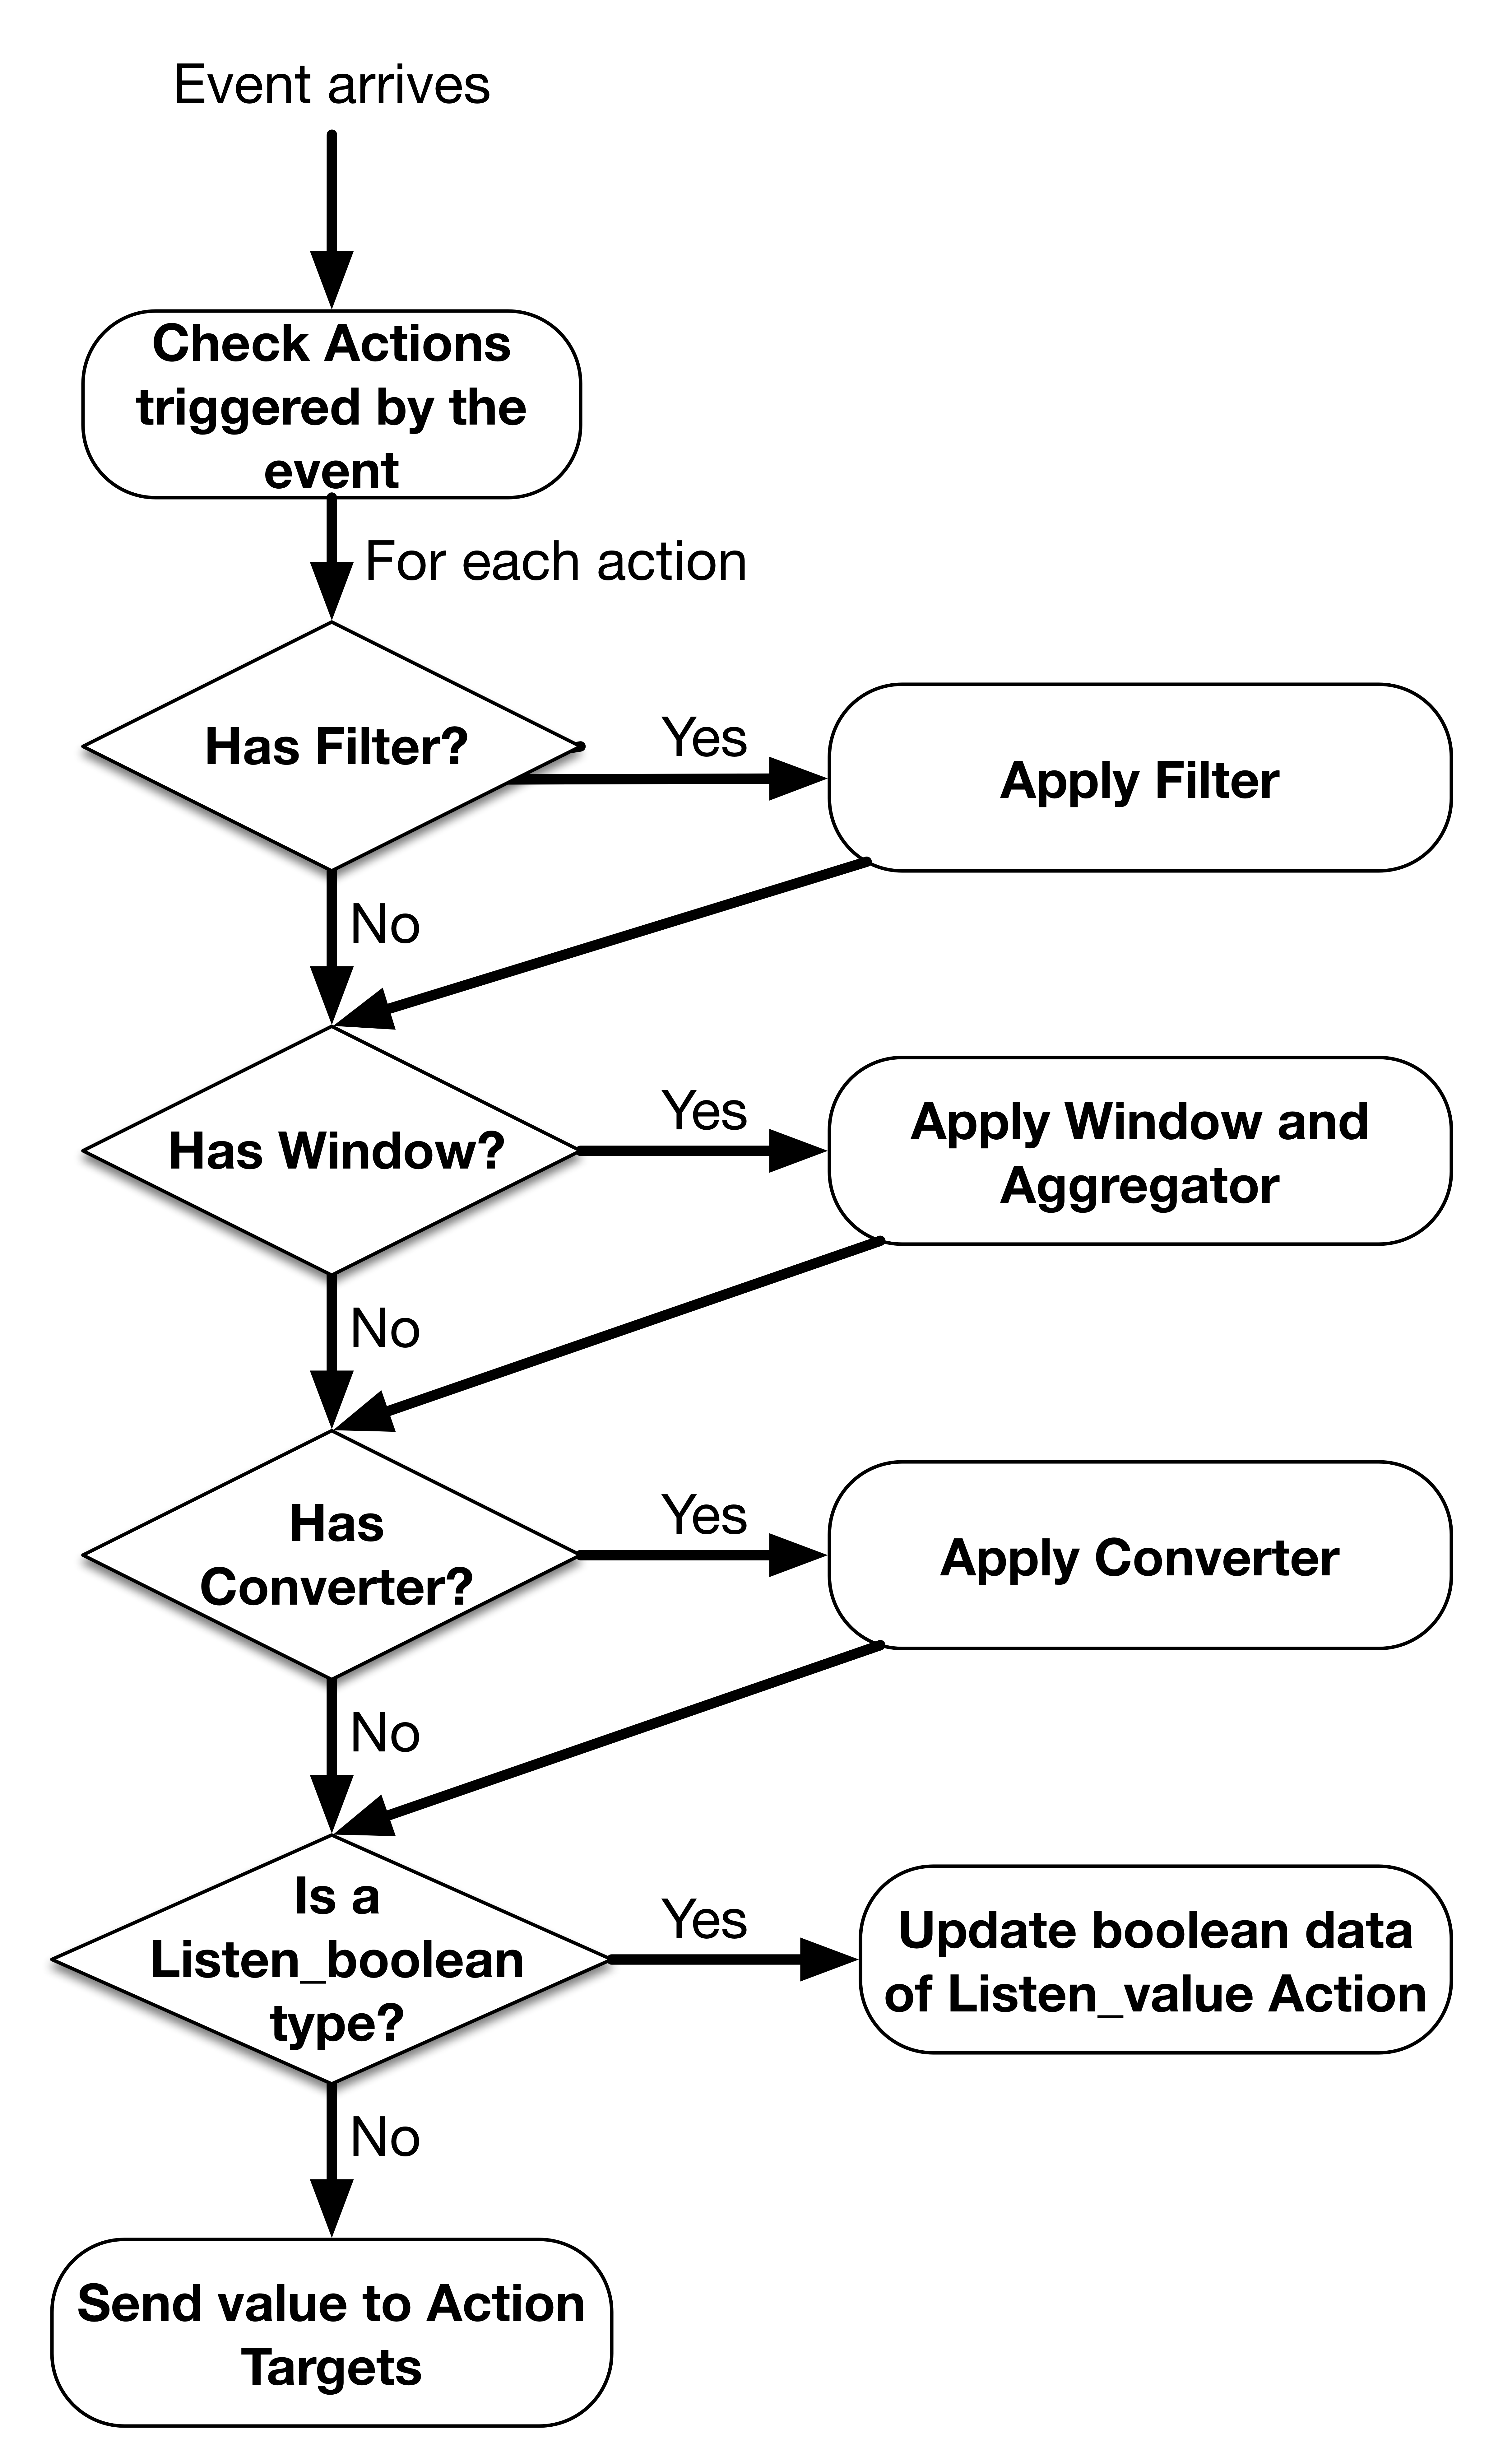
\includegraphics[width=0.7\textwidth]{figures/action.png}
	\caption{Event processing flow diagram.}
	\label{fig:action}
\end{figure}

\end{Paragraph}

\section{Functioning Scenarios}
\label{implementation:scenarios}

As one of the most important requirements and objectives for the present dissertation project, the fail handling mechanisms are a core feature for every smart environment deployed in a building. In order to rely with assurance in a fully autonomous system, it must be adapted to answer swiftly to unexpected behaviours within the system. In the scope of this project, the most important component, to impose an autonomous system, is the \ac{cep} engine, however if that component fails, due to internal software failure or a communication failure, the integrity of the building as well as the safety of its occupants could be at risk. For this reason, as addressed before, an automation engine (\ac{gae}) was implemented so that gateways could process events in order to trigger actions.

In Section \ref{Architecture:usecases}, were introduced three different functioning scenarios: one with every component working as expected, other with the \ac{cep} Engine down and lastly, one with the broker down. However, since a new component was introduced, the Gateway Manager, two new scenarios of failure emerged. Since the Gateway Manager is responsible for failure handling gateways, if a gateway fails while this component is down, the lost devices and rules will not be distributed to other gateways.

\begin{Paragraph}{Functioning scenario 1}
\begin{figure}[H]
	\centering
	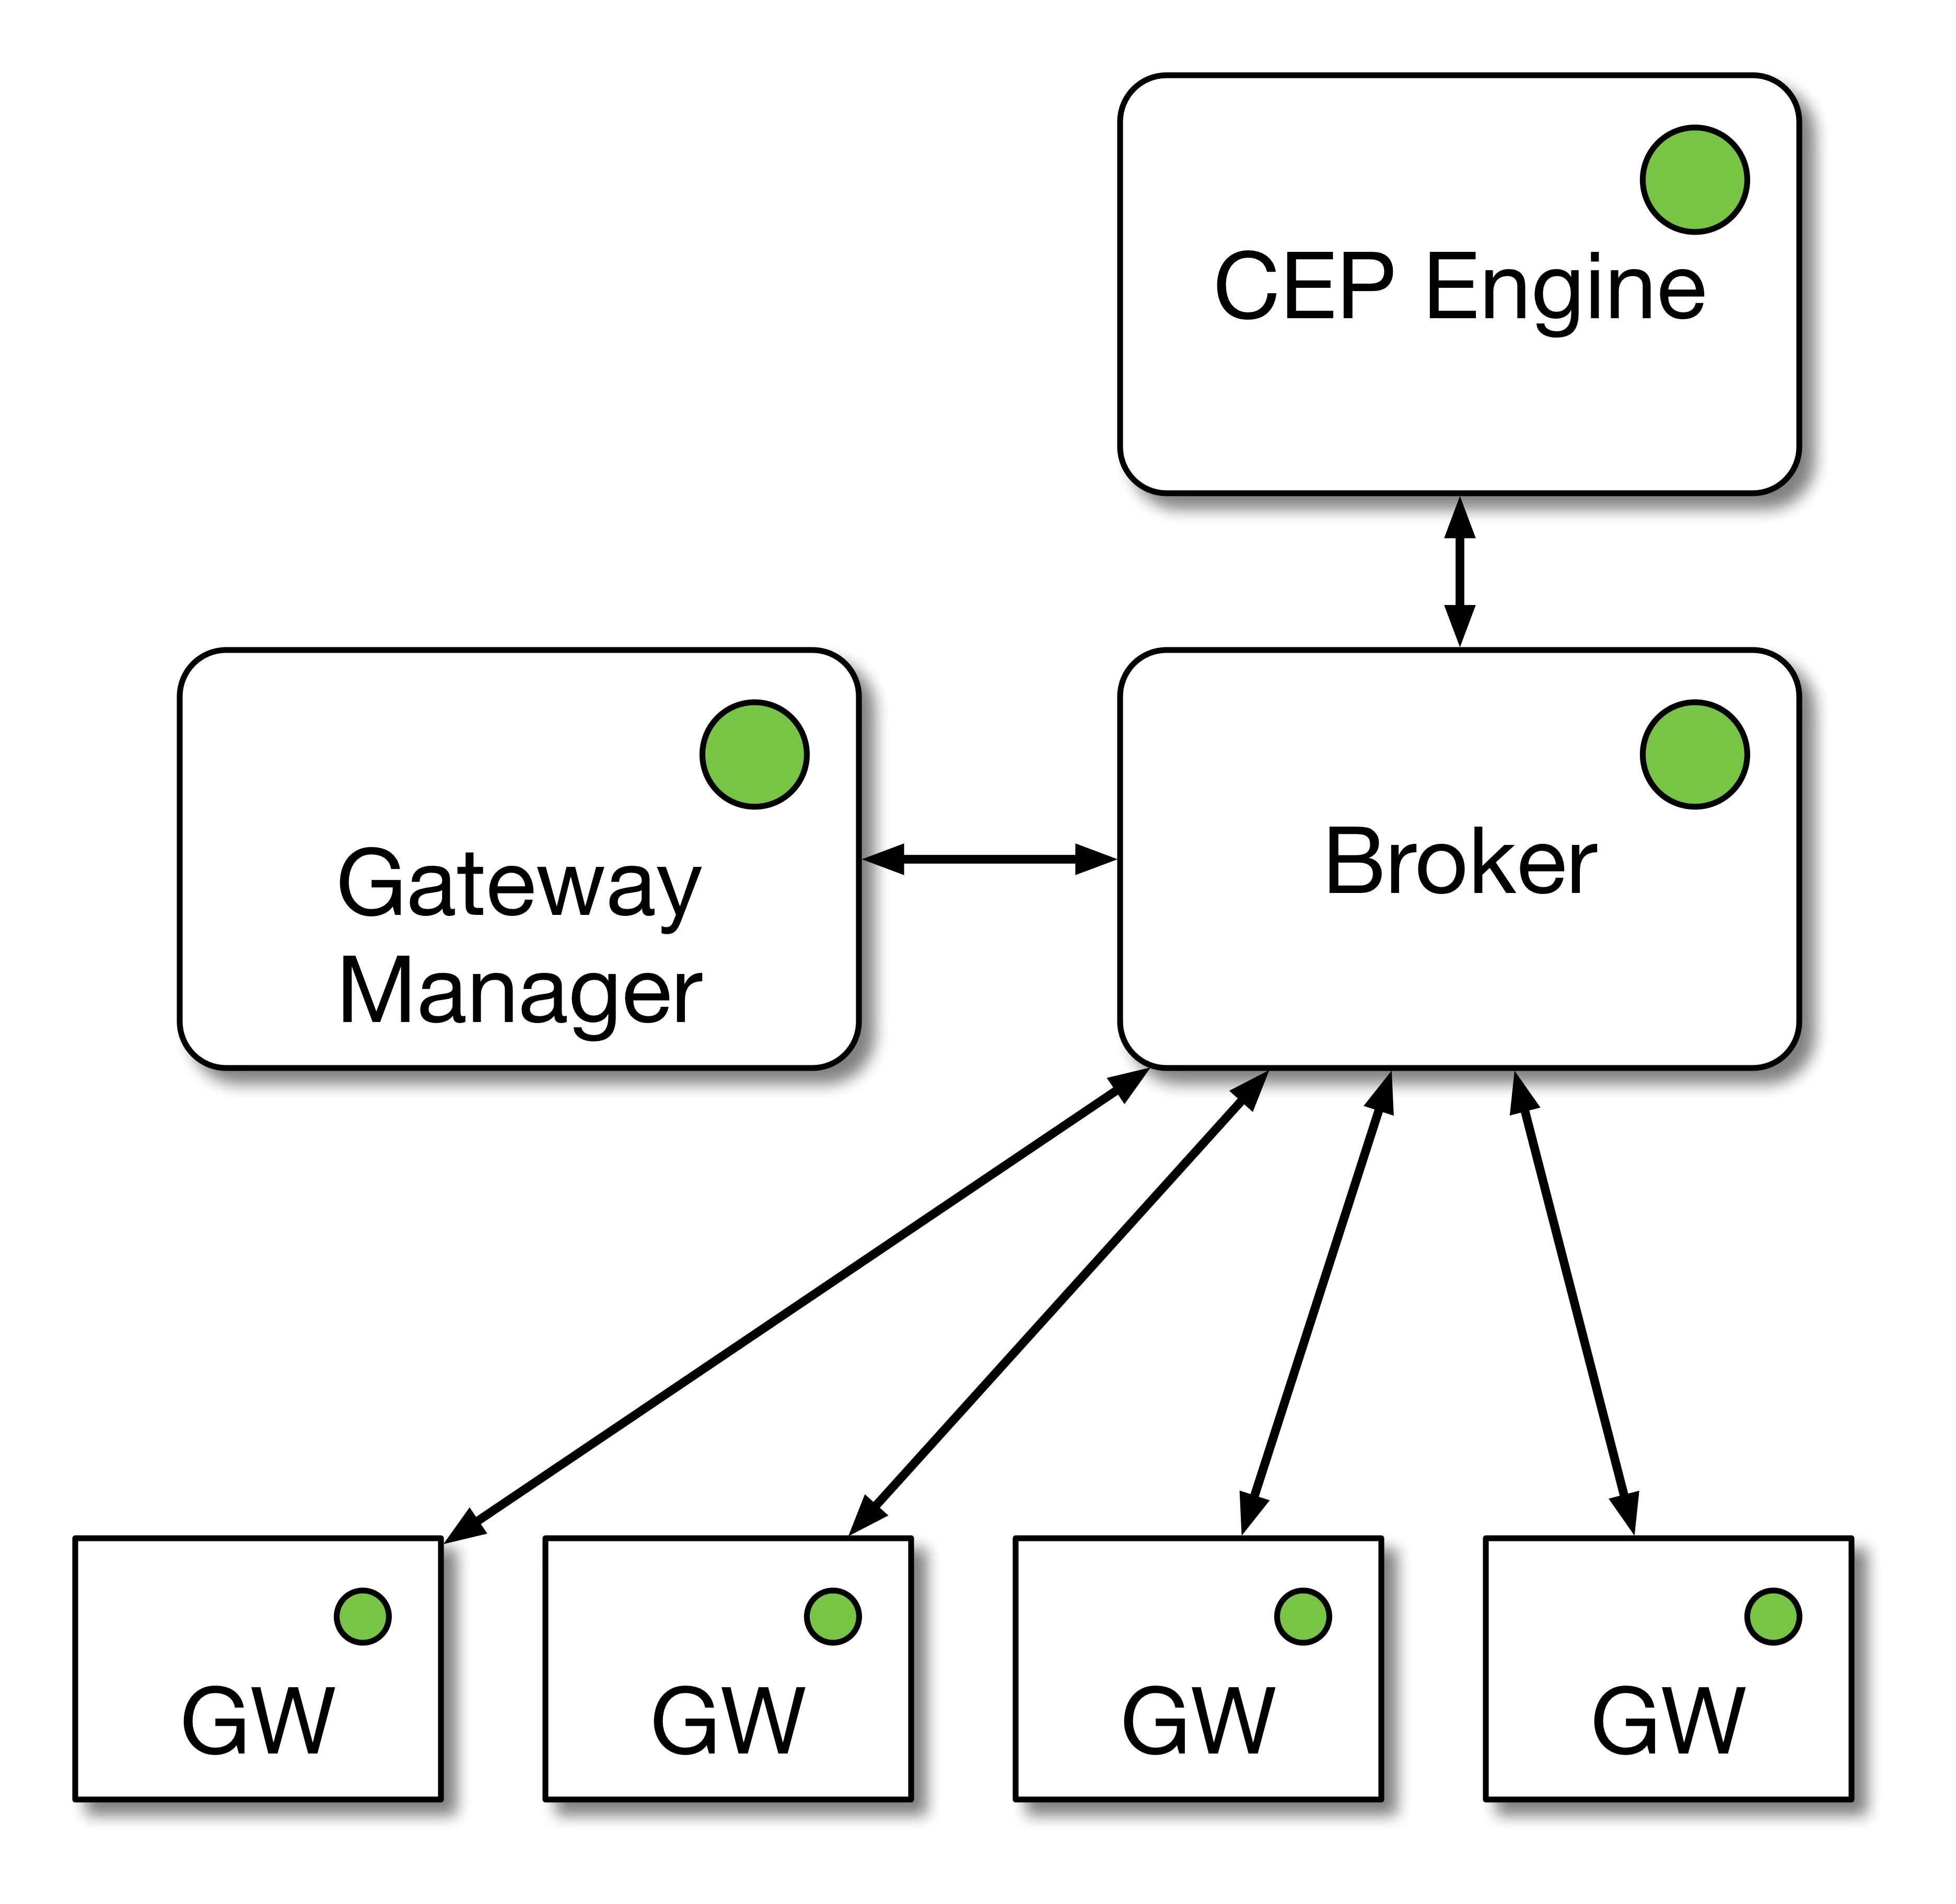
\includegraphics[width=0.6\textwidth]{figures/fs1.png}
	\caption{Functioning scenario 1.}
	\label{fig:fs1}
\end{figure}
\end{Paragraph}

\begin{Paragraph}{Functioning scenario 2}
\begin{figure}[H]
	\centering
	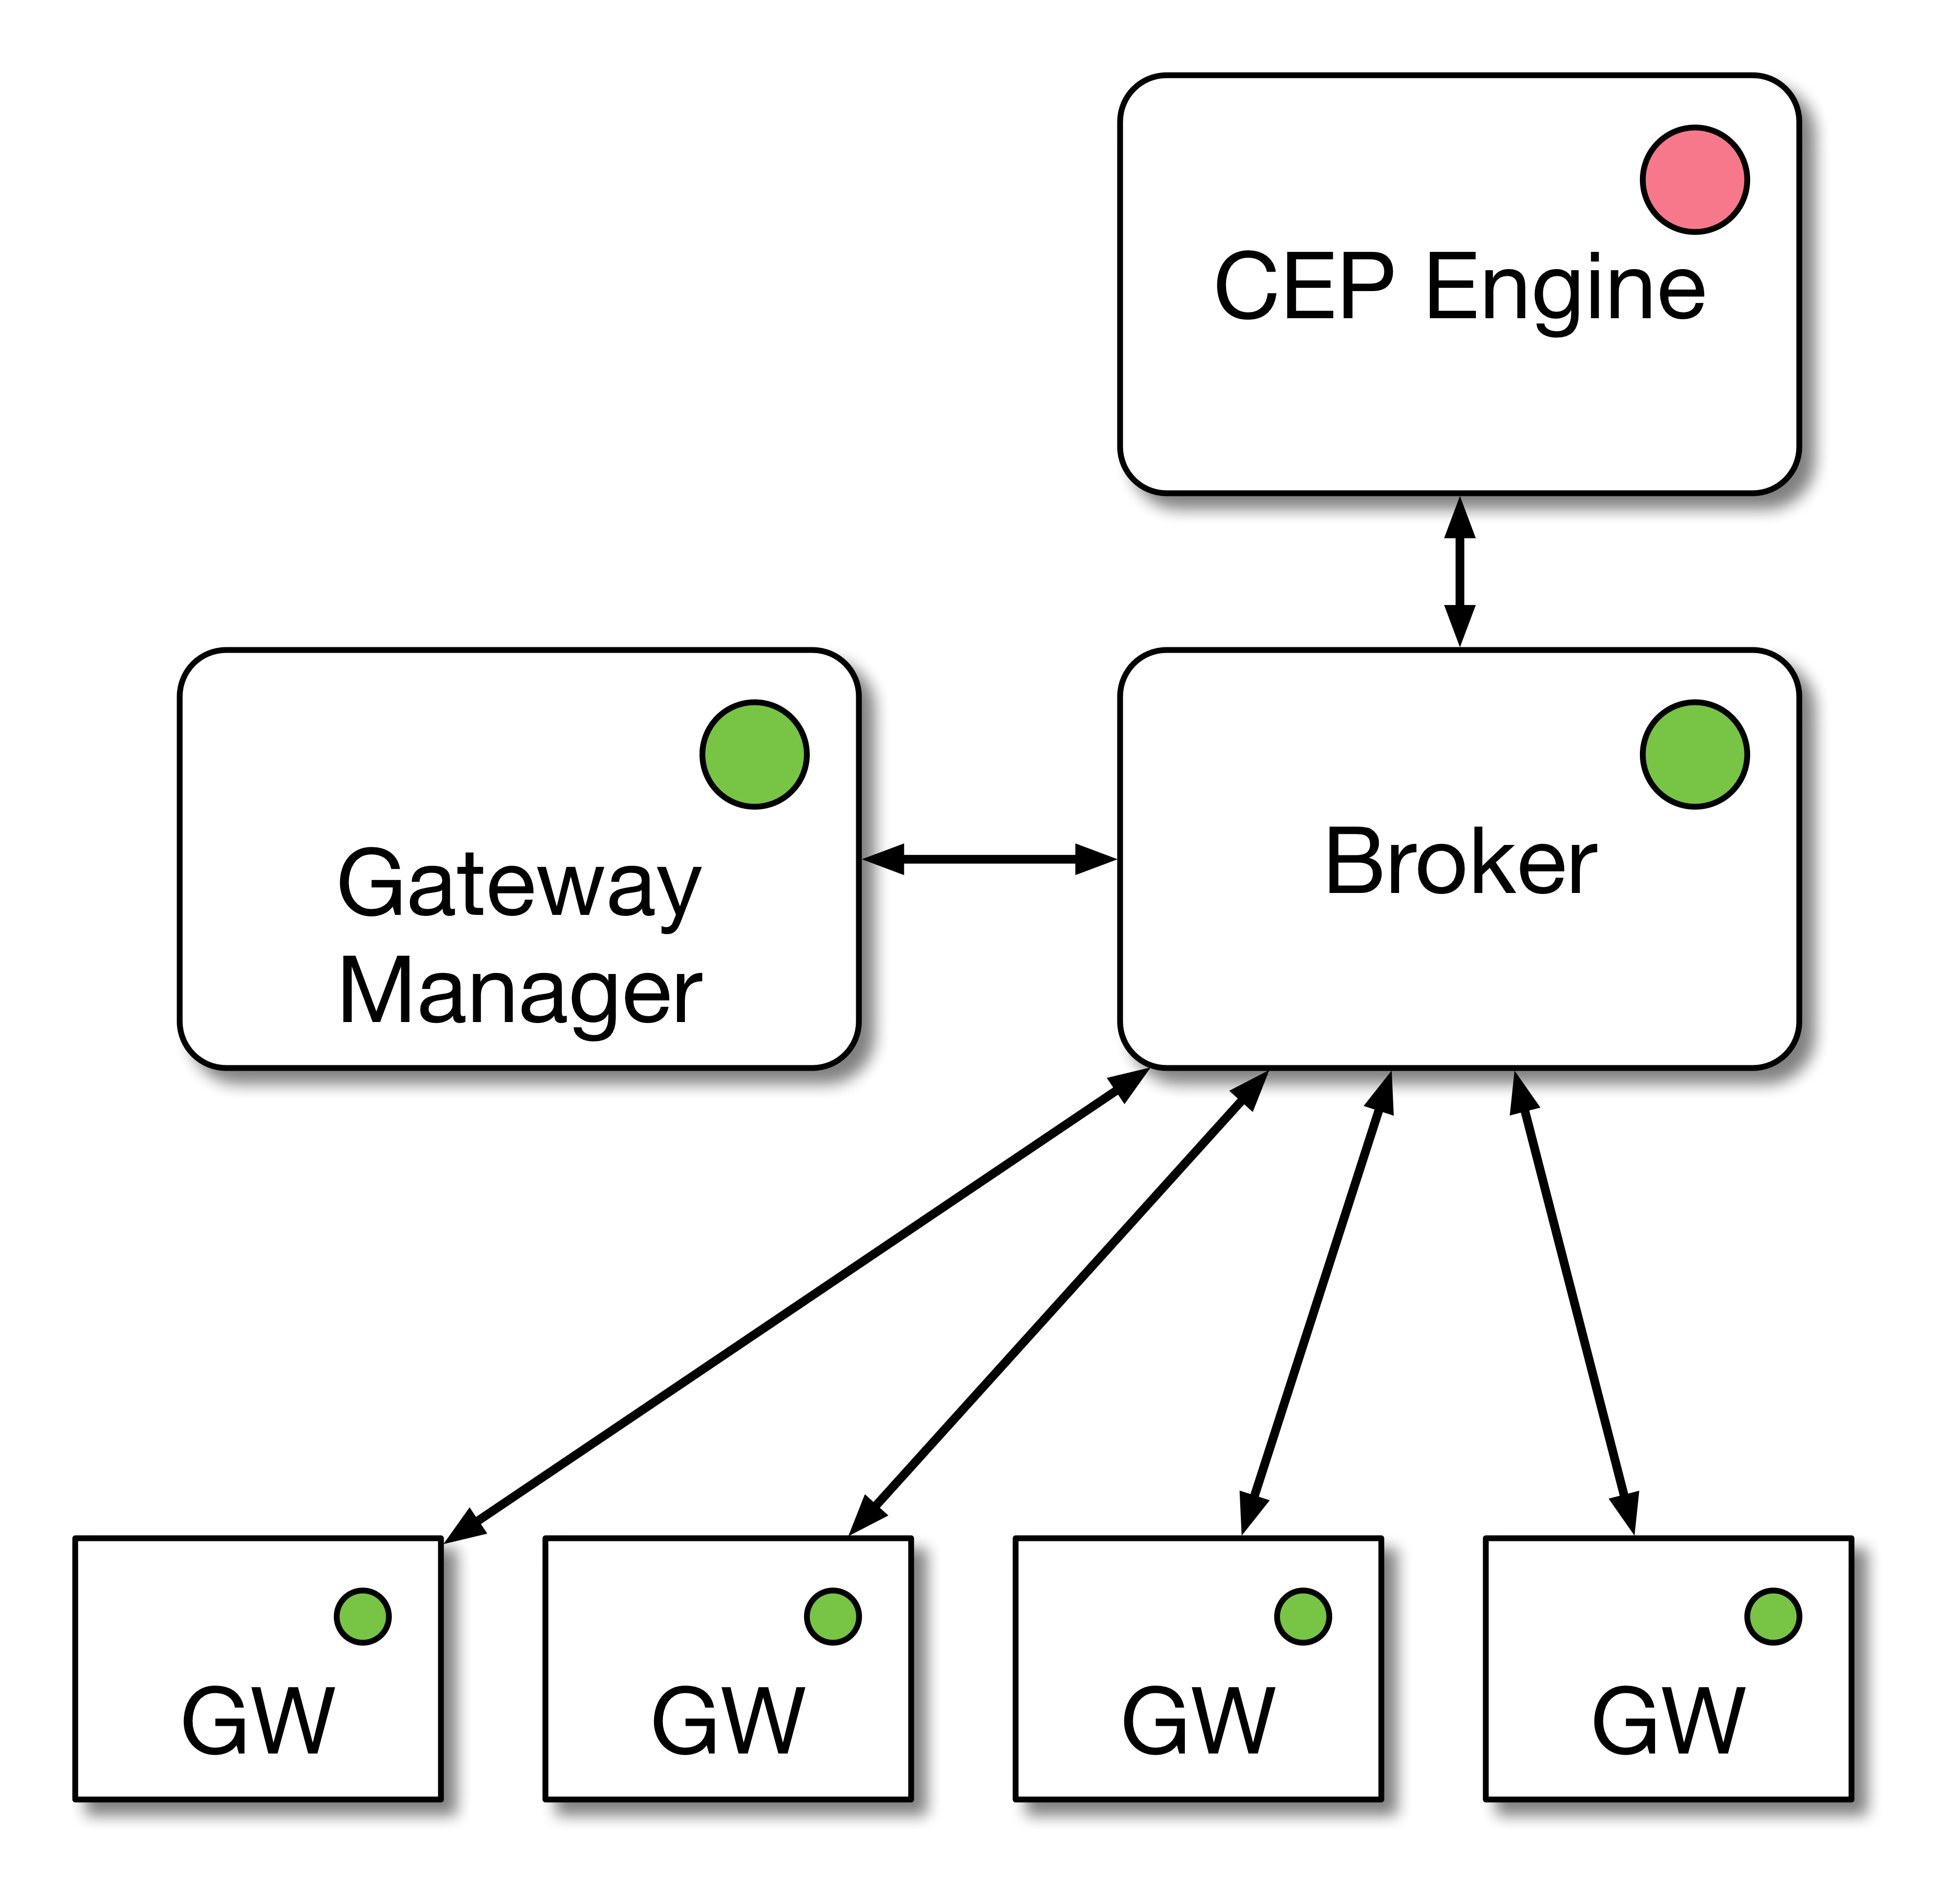
\includegraphics[width=0.6\textwidth]{figures/fs2.png}
	\caption{Functioning scenario 2.}
	\label{fig:fs2}
\end{figure}
\end{Paragraph}

\begin{Paragraph}{Functioning scenario 3}
\begin{figure}[H]
	\centering
	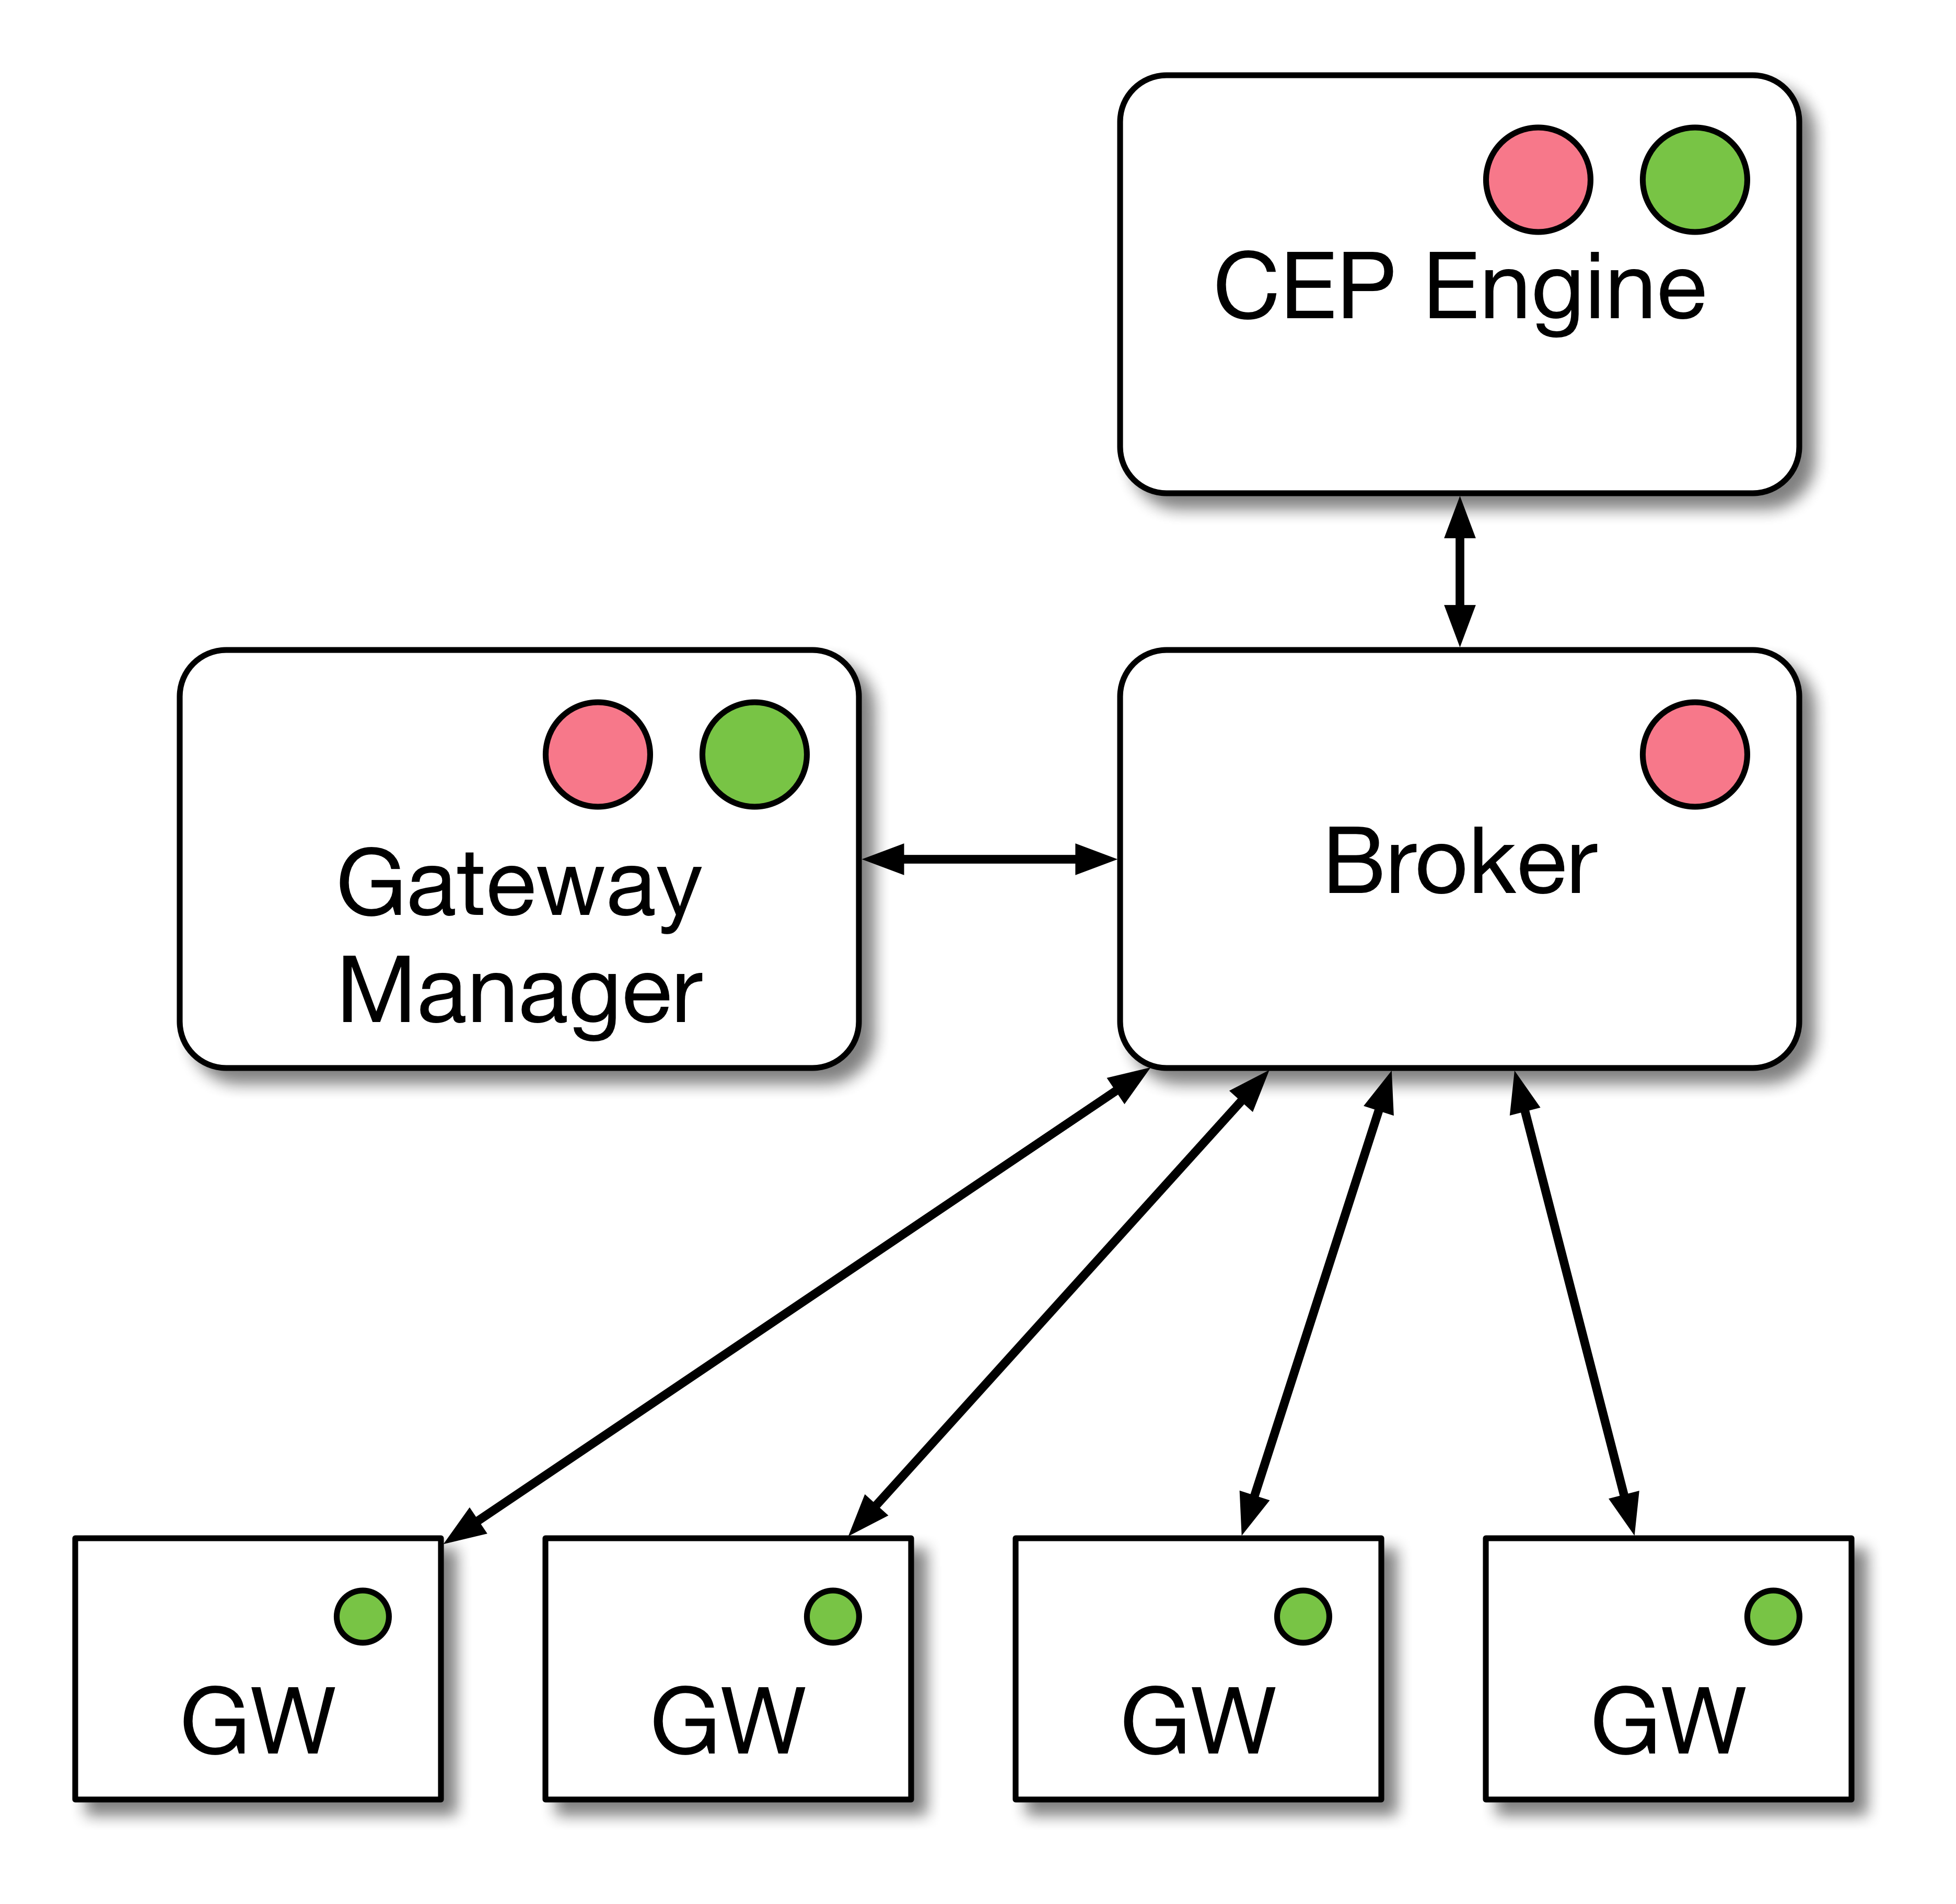
\includegraphics[width=0.6\textwidth]{figures/fs3.png}
	\caption{Functioning scenario 3.}
	\label{fig:fs3}
\end{figure}
\end{Paragraph}

\begin{Paragraph}{Functioning scenario 4}
\begin{figure}[H]
	\centering
	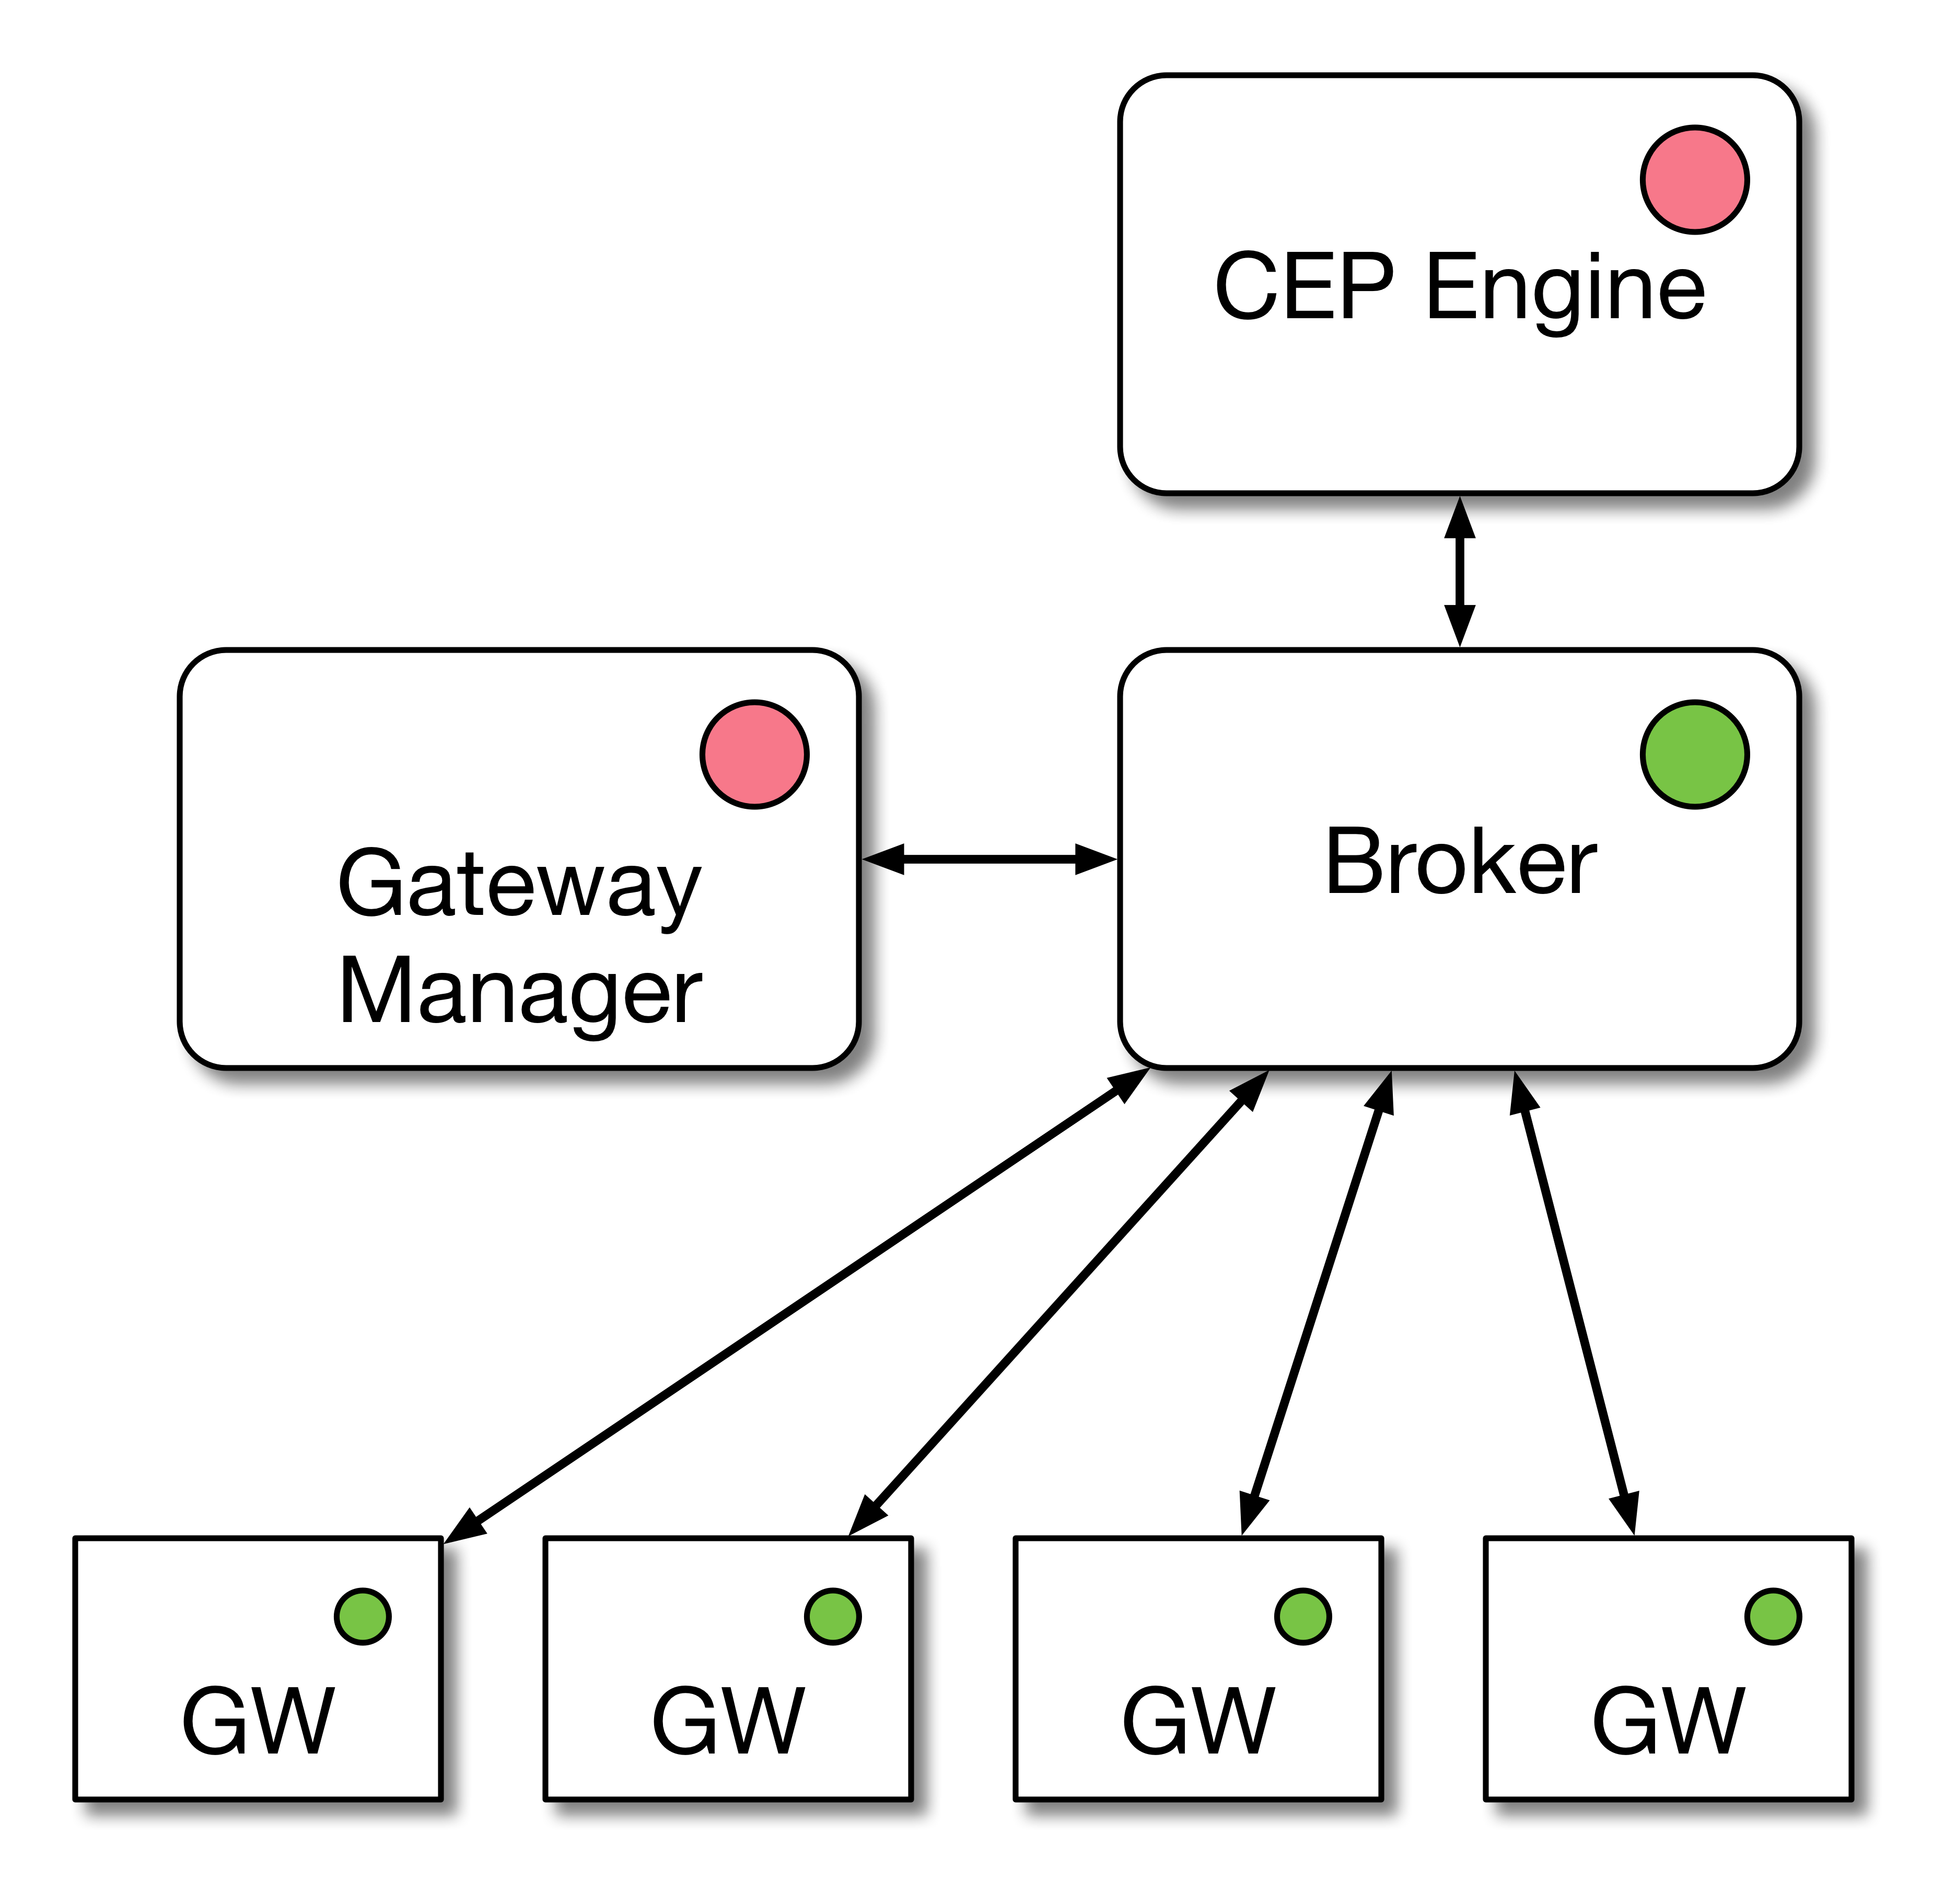
\includegraphics[width=0.6\textwidth]{figures/fs4.png}
	\caption{Functioning scenario 4.}
	\label{fig:fs4}
\end{figure}
\end{Paragraph}

\begin{Paragraph}{Functioning scenario 5}
\begin{figure}[H]
	\centering
	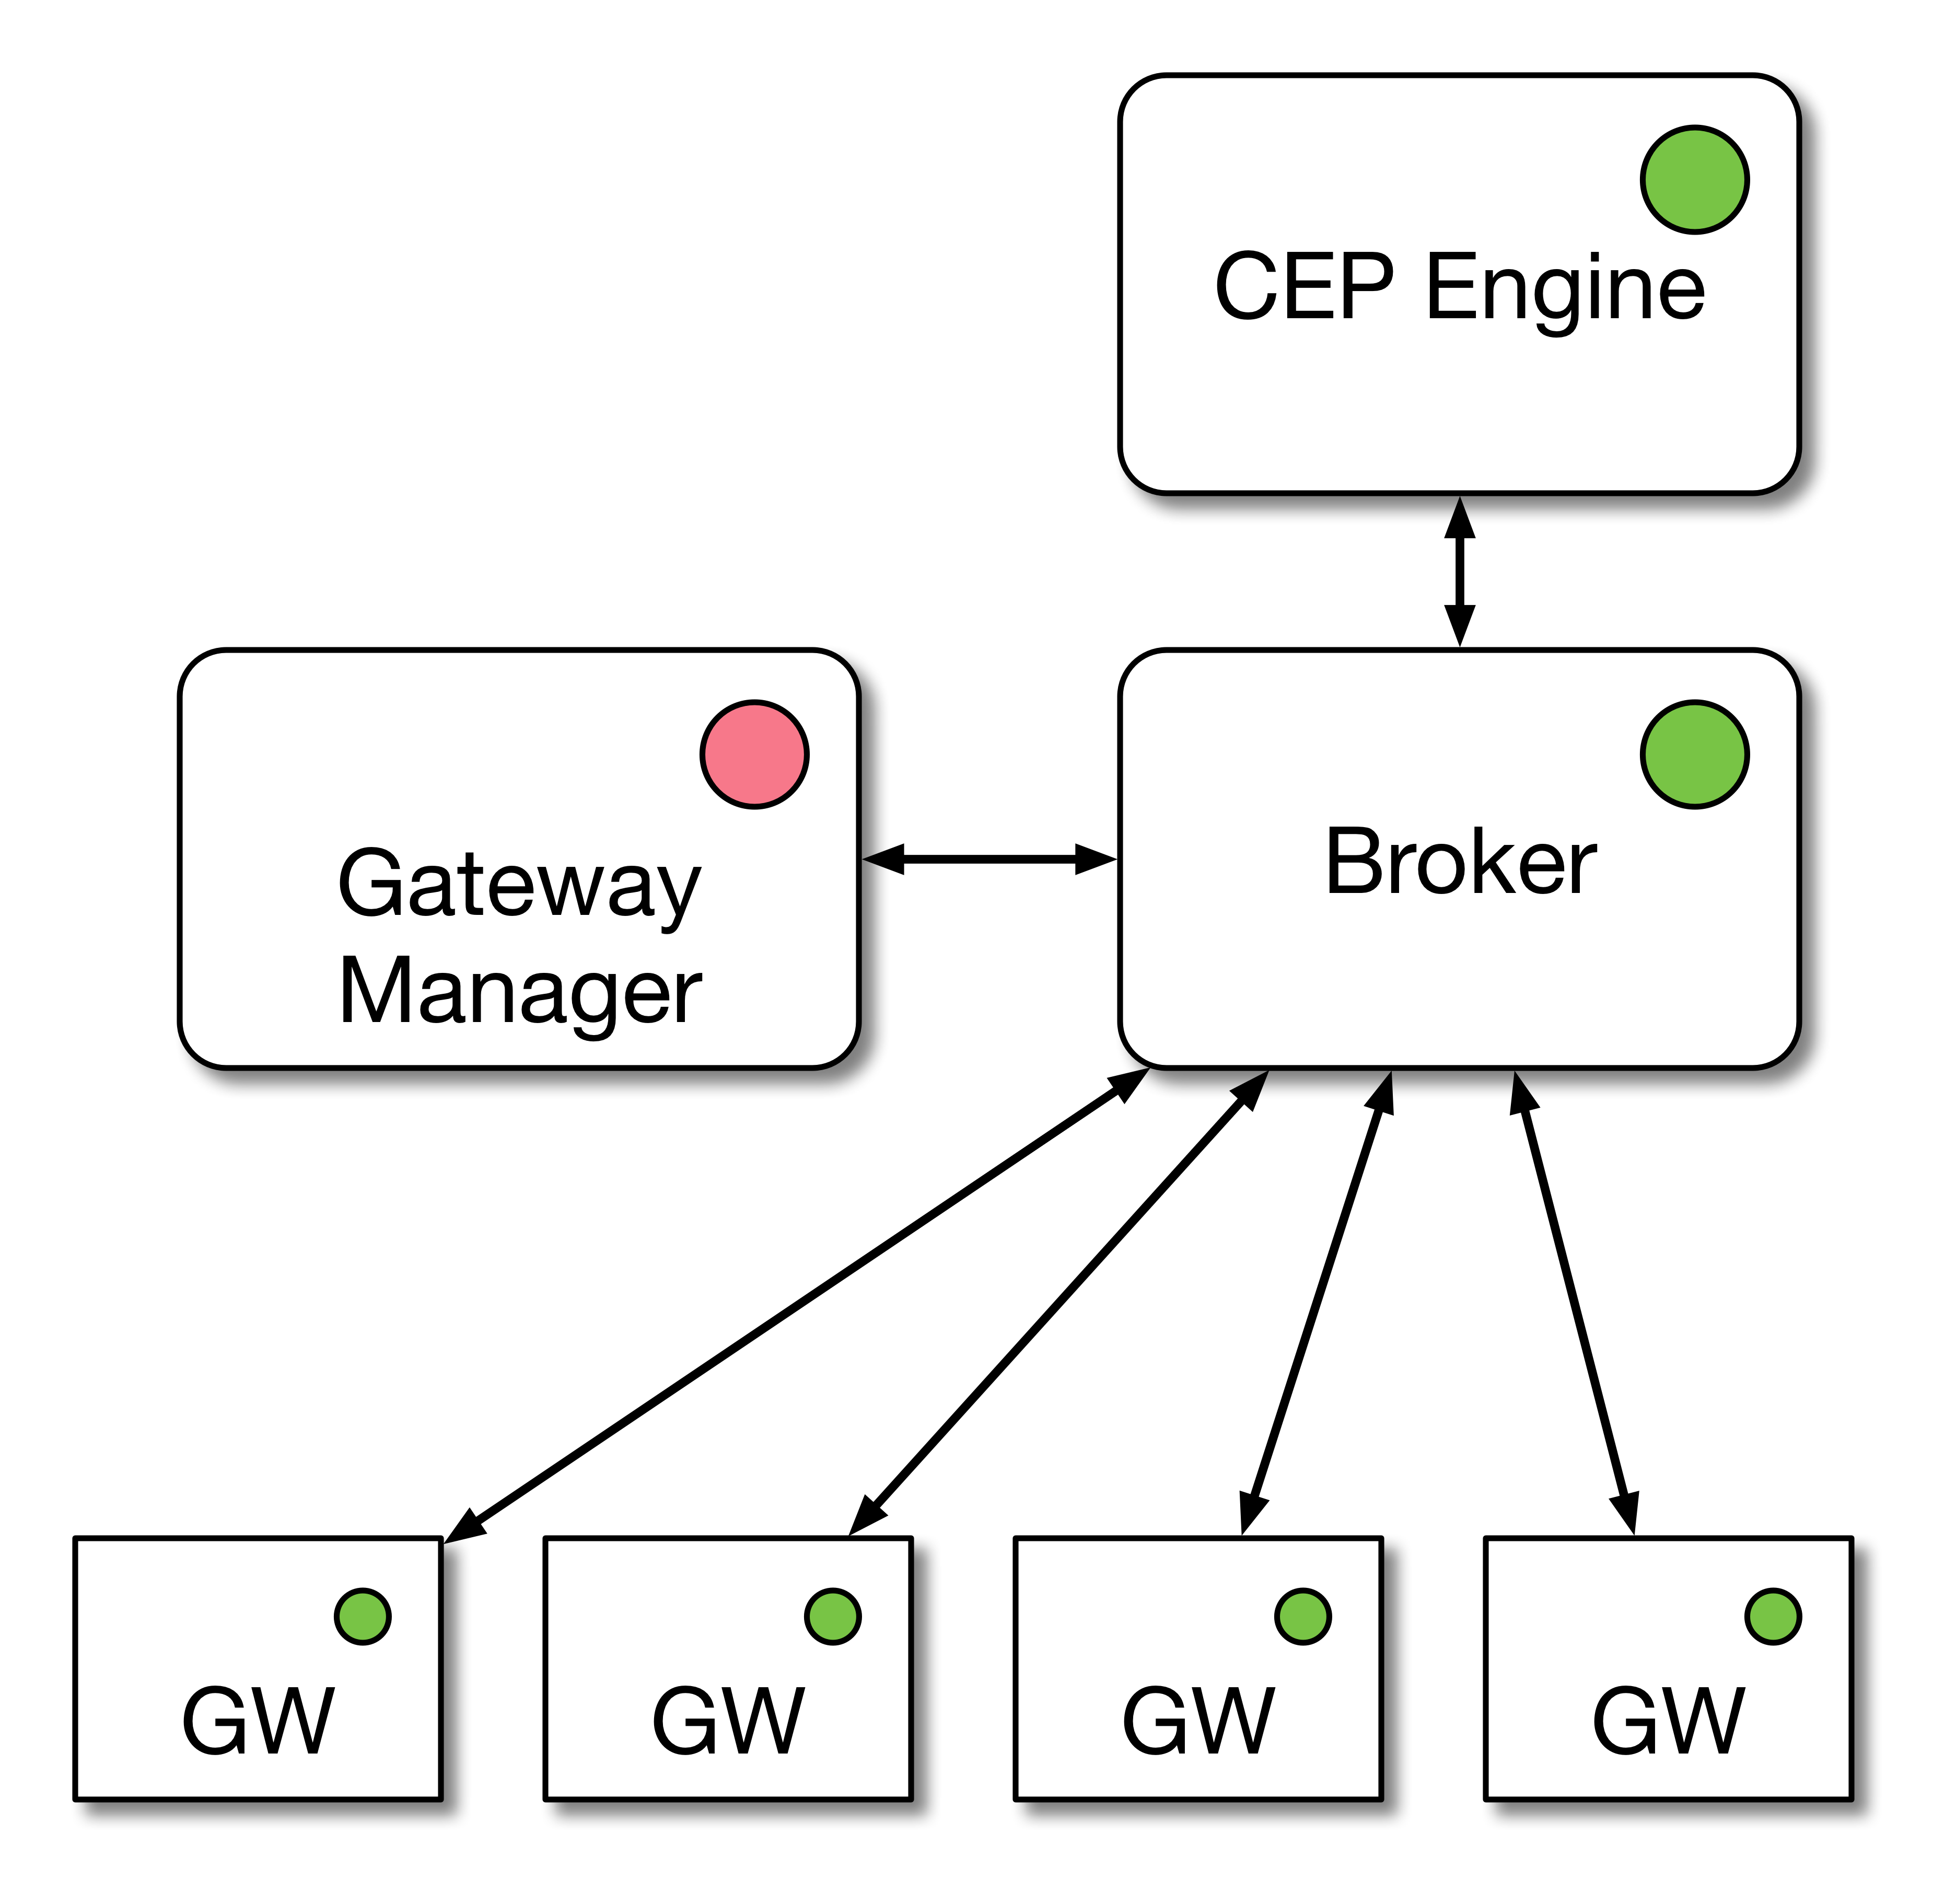
\includegraphics[width=0.6\textwidth]{figures/fs5.png}
	\caption{Functioning scenario 5.}
	\label{fig:fs5}
\end{figure}
\end{Paragraph}


